% LaTeX Document Class for Doctoral Thesis
% Universidad de Alcalá
% Version 1.0
%
% Gracias a: Alvaro Quintanar, Macias, Javier, y a todos los que han colaborado
% en la creación de este documento.

% Modificado por: David Carrascal {david.carrascal@uah.es}

\documentclass[11pt,a4paper,openright,twoside]{book}
% JLD: Esta opcion corresponde al texto para publicar online
%\documentclass[11pt,a4paper,openright]{book}

% Define una geometría de página cuidada y adecuada para impresión
\usepackage[DIV=12,BCOR=12mm,headinclude=true,footinclude=false]{typearea}

%Para corregir los margenes de paginas pares e impares para impresion a dos caras. Sin esto salen al reves.
\let\tmp\oddsidemargin
\let\oddsidemargin\evensidemargin
\let\evensidemargin\tmp
\reversemarginpar

%Para agrandar un poco el margen superior y empequeñecer el inferior, que me parecia estaban un poco descompensados
\voffset=0.5cm

% Añade al índice y numera hasta la profundidad 4.
% 1:section,2:subsection,3:subsubsection,4:paragraph
\setcounter{tocdepth}{4}
\setcounter{secnumdepth}{4}

%%%%%%%%%%%%%%%%%%%%%%%%
% BIBLIOGRAFÍA
%%%%%%%%%%%%%%%%%%%%%%%%
\usepackage[numbers]{natbib}
\usepackage{breakcites,notoccite}

%%%%%%%%%%%%%%%%%%%%%%%%
% DOCUMENTO EN ESPAÑOL
%%%%%%%%%%%%%%%%%%%%%%%%
\usepackage[spanish]{babel}
\usepackage[utf8]{inputenc}
\usepackage[T1]{fontenc}

%%%%%%%%%%%%%%%%%%%%%%%% 
% COLORES
%%%%%%%%%%%%%%%%%%%%%%%% 
% Biblioteca de colores
\usepackage{color}
\usepackage[table,xcdraw,dvipsnames]{xcolor}
% Otros colores definidos por el usuario
\definecolor{gray97}{gray}{.97}
\definecolor{gray75}{gray}{.75}
\definecolor{gray45}{gray}{.45}
\definecolor{gray30}{gray}{.30}
\definecolor{negro}{RGB}{0,0,0}
\definecolor{blanco}{RGB}{255,255,255}
\definecolor{dkgreen}{rgb}{0,.6,0}
\definecolor{dkblue}{rgb}{0,0,.6}
\definecolor{dkyellow}{cmyk}{0,0,.8,.3}
\definecolor{gray}{rgb}{0.5,0.5,0.5}
\definecolor{mauve}{rgb}{0.58,0,0.82}
\definecolor{deepblue}{rgb}{0,0,0.5}
\definecolor{deepred}{rgb}{0.6,0,0}
\definecolor{deepgreen}{rgb}{0,0.5,0}
\definecolor{MyDarkGreen}{rgb}{0.0,0.4,0.0}
\definecolor{bluekeywords}{rgb}{0.13,0.13,1}
\definecolor{greencomments}{rgb}{0,0.5,0}
\definecolor{redstrings}{rgb}{0.9,0,0}
\definecolor{pantone293}{RGB}{35,91,168}

%%%%%%%%%%%%%%%%%%%%%%%%
% TABLAS
%%%%%%%%%%%%%%%%%%%%%%%%
% Paquetes para tablas
\usepackage{longtable,booktabs,array,multirow,multicol,tabularx,ragged2e,array}
\usepackage{graphicx}

% Nuevos tipos de columna para tabla, se pueden utilizar como por ejemplo C{3cm} en la definición de columnas de la función tabular
\newcolumntype{L}[1]{>{\raggedright\let\newline\\\arraybackslash\hspace{0pt}}m{#1}}
\newcolumntype{C}[1]{>{\centering\let\newline\\\arraybackslash\hspace{0pt}}m{#1}}
\newcolumntype{R}[1]{>{\raggedleft\let\newline\\\arraybackslash\hspace{0pt}}m{#1}}

%%%%%%%%%%%%%%%%%%%%%%%% 
% GRAFICAS y DIAGRAMAS 
%%%%%%%%%%%%%%%%%%%%%%%% 
% Paquete para todo tipo de gráficas, diagramas, modificación de imágenes, etc
\usepackage{rotating}
\usepackage{tikz,tikzpagenodes}
\usetikzlibrary{tikzmark,calc,shapes.geometric,arrows, arrows.meta,backgrounds,shadings,shapes.arrows,shapes.symbols,shadows,positioning,fit,automata,patterns,intersections}


\usepackage{pgfplots}
\pgfplotsset{colormap/jet}
\pgfplotsset{compat=newest} % Compatibilidad
\usepgfplotslibrary{patchplots,groupplots,fillbetween,polar}
\usepackage{pgfplotstable}

%%%%%%%%%%%%%%%%%%%%%%%% 
% FIGURAS, TABLAS, ETC 
%%%%%%%%%%%%%%%%%%%%%%%% 
\usepackage{subcaption} % Para poder realizar subfiguras
\usepackage{caption} % Para aumentar las opciones de diseño
% Nombres de figuras, tablas, etc, en negrita la numeración, todo con letra small
\captionsetup{labelfont={bf,small},textfont=small}
% Paquete para modificar los espacios arriba y abajo de una figura o tabla
\usepackage{setspace}
% Define el espacio tanto arriba como abajo de las figuras, tablas
\setlength{\intextsep}{5mm}
% Para ajustar tamaños de texto de toda una tabla o grafica
% Uso: {\scalefont{0.8} \begin{...} \end{...} }
\usepackage{scalefnt}


%%%%%%%%%%%%%%%%%%%%%%%% 
% OTROS
%%%%%%%%%%%%%%%%%%%%%%%%
% Para hacer una pagina horizontal. Uso: \begin{landscape} xxxx \end{lanscape}
\usepackage{lscape}
% Para incluir paginas PDF. Uso:
% \includepdf[pages={1}]{tuarchivo.pdf}
\usepackage{pdfpages}
% Para introducir url's con formato. Uso: \url{http://www.google.es}
\usepackage{url}
% Paquete que añade el hipervinculo en referencias dentro del documento, indice, etc
% Se define sin bordes alrededor. Uso: \ref{tulabel}
\usepackage[pdfborder={000}]{hyperref}
\usepackage{float}
\usepackage{placeins}
\usepackage{afterpage}
\usepackage{verbatim}

%%%%%%%%%%%%%%%%%%%%%%%% 
% GLOSARIOS
%%%%%%%%%%%%%%%%%%%%%%%%
\usepackage[acronym,nonumberlist,toc]{glossaries}
\usepackage{glossary-superragged}
\newglossarystyle{modsuper}{%
  \setglossarystyle{super}%
  \renewcommand{\glsgroupskip}{}
}
\renewcommand{\glsnamefont}[1]{\textbf{#1}}


%%%%%%%%%%%%%%%%%%%%%%%% 
% MATEMÁTICAS Y ALGORITMOS
%%%%%%%%%%%%%%%%%%%%%%%%
\usepackage{mathtools,amsthm,amsfonts,amssymb,bm,mathrsfs,nicefrac,upgreek,bigints}
\usepackage[linesnumbered,ruled,vlined,spanish]{algorithm2e}

%%%%%
% PARÁMETROS DE FORMATO DE CODIGOS
%%%%%
% Puedes editar los formatos para ajustarlos a tu gusto
%%%%%%%%%%%%%%%%%%%%%%%% 
% CÓDIGO. CONFIGURACIÓN. En el siguiente bloque están los estilos.
%%%%%%%%%%%%%%%%%%%%%%%%
% Paquete para mostrar código de matlab. En caja y lineas numeradas
\usepackage[framed,numbered]{matlab-prettifier}
% Paquete mostrar código de programación de distintos lenguajes

\usepackage{listings}
\lstset{ inputencoding=utf8,
extendedchars=true,
frame=single, % Caja donde se ubica el código
backgroundcolor=\color{gray97}, % Color del fondo de la caja
rulesepcolor=\color{black},
boxpos=c,
abovecaptionskip=-4pt,
aboveskip=12pt,
belowskip=0pt,
lineskip=0pt,
framerule=0pt,
framextopmargin=4pt,
framexbottommargin=4pt,
framexleftmargin=11pt,
framexrightmargin=0pt,
linewidth=\linewidth,
xleftmargin=\parindent,
framesep=0pt,
rulesep=.4pt,
stringstyle=\ttfamily,
showstringspaces = false,
showspaces = false,
showtabs = false,
columns=fullflexible,
basicstyle=\small\ttfamily,
commentstyle=\color{gray45},
keywordstyle=\bfseries,
tabsize=4,
numbers=left,
numbersep=1pt,
numberstyle=\tiny\ttfamily\color{gray75},
numberfirstline = false,
breaklines=true,
postbreak=\mbox{\textcolor{red}{$\hookrightarrow$}\space}, % Flecha al saltar de linea
prebreak=\mbox{\textcolor{red}{$\hookleftarrow$}\space}, % Flecha al saltar de linea
literate=
  {á}{{\'a}}1 {é}{{\'e}}1 {í}{{\'i}}1 {ó}{{\'o}}1 {ú}{{\'u}}1
  {Á}{{\'A}}1 {É}{{\'E}}1 {Í}{{\'I}}1 {Ó}{{\'O}}1 {Ú}{{\'U}}1
  {à}{{\`a}}1 {è}{{\`e}}1 {ì}{{\`i}}1 {ò}{{\`o}}1 {ù}{{\`u}}1
  {À}{{\`A}}1 {È}{{\'E}}1 {Ì}{{\`I}}1 {Ò}{{\`O}}1 {Ù}{{\`U}}1
  {ä}{{\"a}}1 {ë}{{\"e}}1 {ï}{{\"i}}1 {ö}{{\"o}}1 {ü}{{\"u}}1
  {Ä}{{\"A}}1 {Ë}{{\"E}}1 {Ï}{{\"I}}1 {Ö}{{\"O}}1 {Ü}{{\"U}}1
  {â}{{\^a}}1 {ê}{{\^e}}1 {î}{{\^i}}1 {ô}{{\^o}}1 {û}{{\^u}}1
  {Â}{{\^A}}1 {Ê}{{\^E}}1 {Î}{{\^I}}1 {Ô}{{\^O}}1 {Û}{{\^U}}1
  {œ}{{\oe}}1 {Œ}{{\OE}}1 {æ}{{\ae}}1 {Æ}{{\AE}}1 {ß}{{\ss}}1
  {ű}{{\H{u}}}1 {Ű}{{\H{U}}}1 {ő}{{\H{o}}}1 {Ő}{{\H{O}}}1
  {ç}{{\c c}}1 {Ç}{{\c C}}1 {ø}{{\o}}1 {å}{{\r a}}1 {Å}{{\r A}}1
  {€}{{\euro}}1 {£}{{\pounds}}1 {«}{{\guillemotleft}}1
  {»}{{\guillemotright}}1 {ñ}{{\~n}}1 {Ñ}{{\~N}}1 {¿}{{?`}}1,
  }

% Intenta no dividir los códigos en diferentes paginas si es posible
\lstnewenvironment{listing}[1][]
   {\lstset{#1}\pagebreak[0]}{\pagebreak[0]}

% Formato de títulos de los códigos
\DeclareCaptionFont{white}{\color{white}}
\DeclareCaptionFormat{listing}{\colorbox{gray}{\parbox{\textwidth - 2\fboxsep}{#1#2#3}}}
\captionsetup[lstlisting]{format=listing,labelfont=white,textfont=white,font= scriptsize}


%%%%%%%%%%%%%%%%%%%%%%%% 
% CÓDIGO. ESTILOS. Ajústalos a tu gusto
%%%%%%%%%%%%%%%%%%%%%%%%
\DeclareOldFontCommand{\bf}{\normalfont\bfseries}{\mathbf}
\lstdefinestyle{Consola}
	{
	basicstyle=\scriptsize\bf\ttfamily,
	showstringspaces=false,
    commentstyle=\color{deepgreen},
    keywordstyle=\color{blue},
	}

\lstdefinestyle{Consola2}
	{
	basicstyle=\footnotesize\bf\ttfamily,
	showstringspaces=false,
    commentstyle=\color{deepgreen},
    keywordstyle=\color{blue},
	}
	
\lstdefinestyle{C}
	{
	basicstyle=\scriptsize,
	language=C,
	}
\lstdefinestyle{C-color}
	{
  	breaklines=true,
  	language=C,
  	basicstyle=\scriptsize,
  	keywordstyle=\bfseries\color{green!40!black},
  	commentstyle=\itshape\color{purple!40!black},
  	identifierstyle=\color{blue},
  	stringstyle=\color{orange},
    }
\lstdefinestyle{P4-color}
	{
  	breaklines=true,
  	language=C,
  	basicstyle=\scriptsize,
  	keywordstyle=\bfseries\color{green!40!black},
  	commentstyle=\itshape\color{purple!40!black},
  	identifierstyle=\color{blue},
  	stringstyle=\color{orange},
  	morekeywords={%
      action, algorithm, apply, attributes, bytes,
      calculated_field, control, counter, current, default, direct,
      drop, else, false, field_list, field_list_calculation, fields,
      header, header_type, hit, if, input, instance_count, last, latest,
      layout, length, mask, max_length, metadata, meter, min_width, miss
      output_width, packets, parse_error, parser, parser_exception, payload,
      primitive_action, register, result, return, saturating, select,
      signed, static, switch, true, type, update, valid, verify, width}
    }

\lstdefinestyle{CSharp}
	{
	basicstyle=\scriptsize
	language=[Sharp]C,
	escapeinside={(*@}{@*)},
	keywordstyle=\bfseries,
	}
\lstdefinestyle{CSharp-color}
	{
	basicstyle=\scriptsize
	language=[Sharp]C,
	escapeinside={(*@}{@*)},
	commentstyle=\color{greencomments},
	keywordstyle=\color{bluekeywords}\bfseries,
	stringstyle=\color{redstrings},
	}
\lstdefinestyle{C++}
	{
	basicstyle=\scriptsize,
	language=C++,
 	}
 	
\lstdefinestyle{C++-color}
	{
  	breaklines=true,
  	language=C++,
  	basicstyle=\scriptsize,
  	keywordstyle=\bfseries\color{green!40!black},
  	commentstyle=\itshape\color{purple!40!black},
  	identifierstyle=\color{blue},
  	stringstyle=\color{orange},
    }
    
\lstdefinestyle{PHP}
	{
	basicstyle=\scriptsize,
	language=PHP,
	}
	
\lstdefinestyle{PHP-color}
	{
	basicstyle=\scriptsize,
	language=PHP,
	keywordstyle    = \color{dkblue},
  	stringstyle     = \color{red},
  	identifierstyle = \color{dkgreen},
  	commentstyle    = \color{gray},
  	emph            =[1]{php},
  	emphstyle       =[1]\color{black},
  	emph            =[2]{if,and,or,else},
  	emphstyle       =[2]\color{dkyellow}
  }
  
\lstdefinestyle{Matlab}
	{
	basicstyle=\scriptsize,
	language=Matlab,
	numberstyle=\tiny\ttfamily\color{gray75},
	}
	
\lstdefinestyle{Matlab-color}
	{
	style = Matlab-editor,
	basicstyle=\scriptsize,
	numberstyle=\tiny\ttfamily\color{gray75},
	}
	
\lstdefinestyle{Latex}
	{
	language=[LaTeX]{Tex},
    basicstyle=\scriptsize,
    literate={\$}{{{\bfseries\$}}}1,
    alsoletter={\\,*,\&},
    emph =[1]{\\begin,\\end,\\caption,\\label,\\centering,\\FloatBarrier,
              \\lstinputlisting,\\scalefont,\\addplot,\\input,
              \\legend,\\item,\\subitem,\\includegraphics,\\textwidth,
              \\section,\\subsection,\\subsubsection,\\paragraph,
              \\cite,\\citet,\\citep,\\gls,\\bibliographystyle,\\url,
              \\citet*,\\citep*,\\todo,\\missingfigure,\\footnote},
  	emphstyle =[1]\bfseries,
  	emph = [2]{equation,subequations,eqnarray,figure,subfigure,
  			   condiciones,flalign,tikzpicture,axis,lstlisting,
  			   itemize,description
  			   },
  	emphstyle =[2]\bfseries,
    numbers=none,
	}
	
\lstdefinestyle{Latex-color}
	{
	language=[LaTeX]{Tex},
    basicstyle=\scriptsize,
    commentstyle=\color{dkgreen},
    identifierstyle=\color{black},
    literate={\$}{{{\bfseries\color{Dandelion}\$}}}1, % Colorea el simbolo dollar
    alsoletter={\\,*,\&},
    emph =[1]{\\begin,\\end,\\caption,\\label,\\centering,\\FloatBarrier,
              \\lstinputlisting,\\scalefont,\\addplot,\\input,
              \\legend,\\item,\\subitem,\\includegraphics,\\textwidth,
              \\section,\\subsection,\\subsubsection,\\paragraph,
              \\cite,\\citet,\\citep,\\gls,\\bibliographystyle,\\url,
              \\citet*,\\citep*,\\todo,\\missingfigure,\\footnote},
  	emphstyle =[1]\bfseries\color{RoyalBlue},
  	emph = [2]{equation,subequations,eqnarray,figure,subfigure,
  			   condiciones,flalign,tikzpicture,axis,lstlisting,
  			   itemize,description
  			   },
  	emphstyle =[2]\bfseries,
    numbers=none,
	}
\lstdefinestyle{Java}
{
	basicstyle=\scriptsize,
	language=Java,
}

\lstdefinestyle{Java-color}
{
	basicstyle=\scriptsize,
	language=Java,
  	keywordstyle=\color{blue},
  	commentstyle=\color{dkgreen},
  	stringstyle=\color{mauve},
}
\lstdefinestyle{Python}
{
	language=Python,
	basicstyle=\scriptsize,
	otherkeywords={self},  
	keywordstyle=\bfseries,     
	emphstyle=\bfseries,    
	emph={MyClass,__init__},         
}

\lstdefinestyle{Python-color}
{
	language=Python,
	basicstyle=\scriptsize,
	otherkeywords={self},          
	keywordstyle=\bfseries\color{deepblue},
	emph={MyClass,__init__},         
	emphstyle=\bfseries\color{deepred},    
	stringstyle=\color{deepgreen},
}
\lstdefinestyle{R}
{
	language=R,                     
  	basicstyle=\scriptsize,
  	keywordstyle=\bfseries, 
}
\lstdefinestyle{R-color}
{
	language=R,                     
  	basicstyle=\scriptsize,
  	keywordstyle=\bfseries\color{RoyalBlue}, 
  	commentstyle=\color{YellowGreen},
  	stringstyle=\color{ForestGreen}  
}




%%%%%%%%%%%%%%%%%%%%%%%%%%
% Frase celebre
%%%%%%%%%%%%%%%%%%%%%%%%%%
\newenvironment{FraseCelebre}
{\begin{list}{}{%
      \setlength{\leftmargin}{0.5\textwidth}
      % Desplazamos el inicio de
      % los párrafos a la derecha la mitad
      % de la anchura de la línea de texto.
      % Puede que quieras cambiar esto
      % por otra cantidad como '5cm'.
      \setlength{\parsep}{0cm}
      % La separación entre párrafos de la
      % frase o de la fuente es normal, sin
      % espacio extra.
      \addtolength{\topsep}{0.5cm}
      % Aumentamos un poco la separación
      % entre la parte de la fase célebre
      % y los párrafos de alrededor
    }
  }
  {\unskip \end{list}}

\newenvironment{Frase}%
{\item \begin{flushright}\small\em}%
  {\end{flushright}}

\newenvironment{Fuente}%
{\item \begin{flushright}\small}%
  {\end{flushright}}

\newenvironment{bottomparagraph}{\par\vspace*{\fill}}{\clearpage}

% Para que las páginas en blanco no tengan numeración.
\newcommand{\clearemptydoublepage}{\newpage{\pagestyle{empty}\cleardoublepage}}

%%%%%%%%%%%%%%%%%%%%%%%%%%%%
% Configuración del español extra
%%%%%%%%%%%%%%%%%%%%%%%%%%%%
\addto\captionsspanish{%
  \renewcommand{\listtablename}{Índice de tablas}
  \renewcommand{\tablename}{Tabla}
  \renewcommand{\lstlistingname}{Código}
  \renewcommand{\lstlistlistingname}{Índice de Códigos}
  \renewcommand{\glossaryname}{Glosario}
  \renewcommand{\acronymname}{Acrónimos}
  \renewcommand{\bibname}{Bibliografía}
}

%%%%%%%%%%%%%%%%%%%%%%%%%%%%%%
% Encabezados y demás
%%%%%%%%%%%%%%%%%%%%%%%%%%%%%%
\usepackage{fancyhdr}
\pagestyle{fancy}

\fancyhf{} % limpia encabezado y pie

% Encabezado izquierdo (páginas pares): capítulo
\fancyhead[LE]{\scshape \leftmark}

% Encabezado derecho (páginas impares): sección
\fancyhead[RO]{\scshape \rightmark}

% Línea horizontal en el encabezado
\renewcommand{\headrulewidth}{0.2pt}

% Número de página centrado en el pie
\fancyfoot[C]{\thepage}

% Redefinir \chaptermark para que \leftmark muestre "Capítulo N. Título"
\renewcommand{\chaptermark}[1]{%
  \markboth{\chaptername\ \thechapter.\ #1}{}}

% Redefinir \sectionmark para que \rightmark muestre "N.M Sección"
\renewcommand{\sectionmark}[1]{%
  \markright{\thesection\ #1}}

% Fichero paradefinir variables de uso general

\newcommand{\titulotesis}{Contribución a tecnologías habilitantes en redes programables y definidas por software}
\newcommand{\autortesis}{David Carrascal Acebron}
\newcommand{\directoruno}{Elisa Rojas Sánchez}
\newcommand{\directordos}{Diego López Pajares}

%%%%%%%%%%%%%%%%%   Configuración adicional   %%%%%%%%%%%%%%%%%%

% Información añadida a las propiedades del archivo PDF.
\hypersetup{
pdfauthor = {David Carrascal~(david.carrascal@uah.es)},
pdftitle = {\titulotesis},
colorlinks=true,     
urlcolor=RoyalBlue,
linkcolor=Black,
filecolor=Black, 
citecolor=RoyalBlue,
}

% Archivo de acrónimos
\makeglossaries
%\makenoidxglossaries 
\newacronym{ieee}{IEEE}{Institute of Electrical and Electronics Engineers}
\newacronym{sdn}{SDN}{Software-Defined Networking}
\newacronym{5g}{5G}{fifth-generation mobile networks}
\newacronym{6g}{6G}{sixth-generation mobile networks}
\newacronym{iot}{IoT}{Internet of Things}
\newacronym{iiot}{IIoT}{Idustrial Internet of Things}
\newacronym{sg}{SG}{Smart grid}
\newacronym{arpanet}{ARPANET}{Advanced Research Projects Agency Network}
\newacronym{onf}{ONF}{Open Networking Foundation}
\newacronym{api}{API}{Application Programming Interface}
\newacronym{nfv}{NFV}{Network Functions Virtualization}
\newacronym{ai}{AI}{Artificial Intelligence}
\newacronym{ml}{ML}{Machine Learning}
\newacronym{capex}{CapEx}{Capital Expenditure}
\newacronym{opex}{OpEx}{Operational Expenditure}
\newacronym{qos}{QoS}{Quality of Service}
\newacronym{p4}{P4}{Programming Protocol-Independent Packet Processors}
\newacronym{grpc}{gRPC}{google Remote Procedure Call}




%%%%%%%%%%%%%%%%%% INICIO DEL DOCUMENTO %%%%%%%%%%%%%%%%%%%%%%%%
\begin{document}

% Portada
\thispagestyle{empty}
\large
\begin{center}

  \color{pantone293}

  \centerline{
\includegraphics[height=3cm]{include/img/logo_uah_nombre.pdf}}
  
  \vspace{2cm}

  \huge{Programa de Doctorado en Tecnologías de la Información y las Comunicaciones}

  \vspace{2cm}

  \Huge\textbf{\titulotesis}

  \vspace{5cm}

  \huge{{Tesis Doctoral presentada por}}\\
  \vspace{2mm}
  \huge{\textbf{\autortesis}}

  \vspace{10mm}

  \color{black}
  
\end{center}

\begin{bottomparagraph}
  \begin{center}

    \color{pantone293}

      \huge {2025}
    \color{black}

  \end{center}
\end{bottomparagraph}

\clearemptydoublepage

% Cover
\thispagestyle{empty}
\large
\begin{center}

  \color{pantone293}

  \centerline{
\includegraphics[height=3cm]{include/img/logo_uah_nombre.pdf}}

  \vspace{2cm}

  \huge{Ph.D. Program in Information and Communications Technologies}

  \vspace{2cm}   
  
  \Huge\textbf{\titulotesis}

  \vspace{10mm}
  
  \huge{{Author}}\\
  %\vspace{2mm}
  \huge{\textbf{\autortesis}}


  \vspace{10mm}
  
  \huge {Advisors}

  \textbf{Dr. \directoruno\\
          Dr. \directordos}

  % \LARGE\textbf{\myWorkTypeFull}

  \color{black}
  

\end{center}

\begin{bottomparagraph}
  \begin{center}

    \color{pantone293}
    \huge {Alcalá de Henares\\2025}
    \color{black}

  \end{center}
\end{bottomparagraph}

\clearemptydoublepage

% Ponemos el tamaño de letra a normal.
\normalsize

%DESCOMENTAR SI SE QUIEREN AÑADIR PDFs CON LOS INFORMES
% \clearemptydoublepage
% \includepdf[pages=1]{informes/informeDirector.pdf}
% 
% \clearemptydoublepage
% \includepdf[pages=1]{letters/informeDepartamento.pdf}


% Números romanos hasta el mainmatter.
\frontmatter

% Init
%%%%%%%%%%%% Frase celebre %%%%%%%%%%%%

% Limpiamos el estilo de la página
\thispagestyle{empty}

\vspace*{4cm}

\begin{flushright}
\itshape
``No os preguntarán por mí,\\
que en estos tiempos a nadie le da lustre\\
haber nacido segundón en casa grande;\\
pero si pregunta alguno,\\
bueno será contestarle\\
que, español, a toda vena,\\
amé, reñí, di mi sangre,\\
pensé poco, recé mucho,\\
jugué bien, perdí bastante.\\[0.7em]

Y, porque esa empresa loca que nunca debió tentarme,\\
que, perdiendo ofende a todos,\\
que, triunfando alcanza a nadie,\\
no quise salir del mundo\\
sin poner mi pica en Flandes.\\[0.7em]

¡Por España!\\[0.7em]

Y el que quiera defenderla honrado muera.\\
Y el traidor que la abandone,\\
no tenga quien le perdone,\\
ni en Tierra Santa cobijo,\\
ni una cruz en sus despojos,\\
ni las manos de un buen hijo,\\
para cerrarle los ojos.''
\end{flushright}

\vspace{1em}
\begin{flushright}
\textsc{Hernando de Acuña}
\end{flushright}

%%%%%%%%%%%%%%%%%%%%%%%%%%%%%%%%%
\clearemptydoublepage %salta a nueva página impar

%%%%%%%%%%%% Funding %%%%%%%%%%%%

% Limpiamos el estilo de la página
\thispagestyle{empty}

\vspace*{\fill}

\begin{flushleft}
\begin{minipage}{\textwidth}
%\raggedright
\scriptsize
Este trabajo ha sido parcialmente financiado por la Universidad de Alcalá a través del programa FPI-UAH 2022; por la Comunidad de Madrid mediante los proyectos TAPIR-CM (S2018/TCS-4496), MistLETOE-CM (CM/JIN/2021-006), TUCAN6-CM (TEC-2024/COM-460) y VERANO (CM/DEMG/2024-038); por el MICIU y la Unión Europea NextGenerationEU/PRTR a través del proyecto ADMINISTER (TED2021-131301B-I00); por el Ministerio de Ciencia e Innovación mediante el proyecto ONENESS (PID2020-116361RA-I00); y por el Ministerio de Asuntos Económicos y Transformación Digital y la Unión Europea–NextGenerationEU a través del proyecto UNICO 5G I+D 6G-DATADRIVEN-02, coordinado por la Universidad Carlos III de Madrid.
\end{minipage}
\end{flushleft}

%%%% Funding

% +   Comunidad de Madrid
%     -   TAPIR-CM (S2018/TCS-4496)
%     -   MistLETOE-CM (CM/JIN/2021-006)
%     -   TUCAN6-CM (TEC-2024/COM-460)
%     -   VERANO (CM/DEMG/2024-038)

% +   MICIU y la Unión Europea NextGenerationEU/PRTR
%     -   ADMINISTER (TED2021-131301B-I00)

% +   Spanish Ministry of Science and Innovation 
%     -   ONENESS (PID2020-116361RA-I00)

% +   Spanish Ministry of Economic Affairs and Digital Transformation and the European Union-NextGenerationEU
%     -   UNICO 5G I+D 6G-DATADRIVEN-02 project coordinated by Universidad Carlos III de Madrid.

% +   Este trabajo ha sido parcialmente financiado por la Universidad de Alcalá a través del programa FPI-UAH 2022;

\vspace{1cm}

%%%%%%%%%%%%%%%%%%%%%%%%%%%%%%%%%
\clearemptydoublepage %salta a nueva página impar

%%%%%%%%%%%% Agradecimientos %%%%%%%%%%%%
\chapter*{Agradecimientos}

% Limpiamos el estilo de la página
%\thispagestyle{empty}

\vspace{1cm}

Es increíble cómo pasa el tiempo, y da vértigo echar la vista atrás. Pensar en cómo he llegado hasta aquí, las conferencias a las que he tenido la suerte de asistir, los viajes que he podido realizar, y, sobre todo, en las personas que he conocido por el camino. A menudo se describe el doctorado como un proceso arduo y exigente, y no diré lo contrario, pero, también merece la pena poner en valor todo lo aprendido, lo vivido y las experiencias que me han hecho crecer tanto a nivel personal como profesional.\\
\\
Escribo estas líneas desde Milán, durante mi estancia doctoral junto a Marco Savi, a quien quiero agradecer sinceramente todo el tiempo, dedicación y esfuerzo que me ha brindado. Su apoyo ha hecho que esta etapa sea verdaderamente inolvidable. Esta experiencia no habría sido la misma sin todas las personas maravillosas que he conocido en Italia, que me han hecho sentir como en casa, siempre con una sonrisa y dispuestas a ayudar.\\
\\
Volviendo la mirada a casa, no puedo dejar de agradecer a mis amigos, que han estado siempre a mi lado, apoyándome en cada paso. A mi familia, por su paciencia infinita, por su ayuda constante y por soportarme en los momentos de estrés y agobio de esta ``empresa loca'' que es el doctorado. A mis amigos del LE-34, los que están y los que ya no están, con quienes he compartido tantos cafés, confidencias, comidas y tardes de ``trabajo''. Y, por supuesto, a todos mis compañeros del grupo NetIS, que tras tantos años, más que colegas se han convertido en una segunda familia. Gracias por creer en mí y por acompañarme hasta aquí.\\
\\
Por último, a Elisa y Diego, mis directores de tesis. Gracias por vuestra guía, vuestro apoyo incondicional y por confiar en mí desde el primer momento. En especial a Elisa: si no fuera por aquel correo que me enviaste hace ya más de siete años, ofreciéndome una mini beca de investigación, hoy no estaría escribiendo estas líneas. Gracias por todo lo que me habéis enseñado, por lo que he aprendido con vosotros y por todo lo que aún me queda por aprender.

\vspace{0.5cm}

Sinceramente, mil gracias a todos.



%%%%%%%%%%%%%%%%%%%%%%%%%%%%%%%%%
\clearemptydoublepage %salta a nueva página impar


%%%%%%%%%%%% Resumen %%%%%%%%%%%%

\chapter{Resumen}

La era contemporánea en la cual vivimos se caracteriza en mayor medida por una profunda transformación tecnológica y social, impulsada por la globalización y por el desarrollo de infraestructuras digitales interconectadas que configuran lo que se conoce como el Internet of Everything (IoE). En este nuevo paradigma, emergen redes densas y altamente heterogéneas en las que convergen dispositivos, servicios y plataformas con requerimientos funcionales muy variopintos, integrando no solo redes de comunicaciones, sino también infraestructuras energéticas, industriales y logísticas. Esta complejidad creciente, demanda nuevas metodologías para un control y gestión, que sea en la medida de lo posible, flexible y escalable. En este contexto, las redes softwarizadas y programables se postulan como una elemento tecnológico clave, al permitir una abstracción funcional de la infraestructura subyacente, facilitar su automatización y promover la integración de capacidades de control, así como, la adaptación dinámica de la red, a las necesidades intrinsecas de los nodos de la misma.\\
\\
Esta Tesis contribuye al desarrollo de las redes softwarizadas y programables mediante la propuesta de soluciones orientadas a mejorar la gestión, la resiliencia y la cooperación entre nodos de dichas redes. En primer lugar, se diseñan y evalúan algoritmos de toma de decisiones inteligentes en entornos altamente dinámicos y heterogéneos, con aplicación en dominios como el Internet de las Cosas Industrial (IIoT), las redes eléctricas inteligentes (Smart Grids) y las redes de comunicaciones de nueva generación. Estas soluciones permiten una asignación dinámica de recursos, una adaptación proactiva a las condiciones del entorno y una reducción sustancial en la complejidad de gestión de la red. Además, se ha abordado la integración de modelos de Inteligencia Artificial (AI) con dichos algoritmos, con el fin de potenciar la detección temprana de fallos, lo que se traduce en una mejora significativa de la resiliencia, y la alta disponibilidad de los servicios. En segundo lugar, se propone una arquitectura software modular, orientada a servicios y alineada con estándares actuales, que permite la incorporación de herramientas emergentes, así como mecanismos automatizados con AI, ofreciendo capacidades  de computación tanto en la nube, como en el edge. Esta arquitectura está concebida para proporcionar una infraestructura lógica robusta, interoperable y escalable, capaz de facilitar la orquestación autónoma de servicios distribuidos, orientado a contextos de elevada heterogeneidad tecnológica, como entornos IIoT u otros.

\vspace{0.5cm}

\textbf{Palabras clave}: Redes densas y hetereogeneas, Redes programables y softwarizadas, Algoritmos, Infraestructura Cloud, IoT industrial, Smart grids.


%%%%%%%%%%%%%%%%%%%%%%%%%%%%%%%%%
\clearemptydoublepage %salta a nueva página impar


%%%%%%%%%%%% Abstract %%%%%%%%%%%%
\chapter{Abstract}

The contemporary era is marked by a profound technological and social transformation, driven by globalization and the pervasive deployment of interconnected digital infrastructures that define the Internet of Everything (IoE). Within this emerging paradigm, dense and highly heterogeneous networks are formed, comprising a wide variety of devices, services, and platforms with diverse and demanding functional requirements. These systems integrate not only communication networks, but also energy, industrial, and logistics infrastructures. The increasing complexity of such environments necessitates the adoption of novel methodologies capable of ensuring the flexible and scalable control and management of distributed resources and services. In this context, softwarized and programmable networks have emerged as a pivotal technological solution, enabling functional abstraction of the underlying infrastructure, supporting automation, and fostering the integration of advanced control mechanisms, as well as the dynamic adaptation of network behavior to the intrinsic requirements of its nodes.\\
\\
This Thesis contributes to the advancement of softwarized and programmable networking by proposing solutions designed to enhance the management, resilience, and cooperation between nodes within these infrastructures. Firstly, it presents and evaluates intelligent decision-making algorithms tailored for highly dynamic and heterogeneous environments, with applications in domains such as the Industrial Internet of Things (IIoT), smart grids, and next-generation communication networks. These algorithms facilitate dynamic resource allocation, proactive environmental adaptation, and a significant reduction in network management complexity. Furthermore, the integration of Artificial Intelligence (AI) models into these solutions is explored to enable early fault detection, thus improving system resilience and ensuring high service availability. Secondly, the Thesis proposes a modular, service-oriented software architecture, aligned with current standards and capable of incorporating emerging technologies and AI-driven automation mechanisms. This architecture offers computing capabilities across both cloud and edge infrastructures and is designed to deliver a robust, interoperable, and scalable logical platform that supports the autonomous orchestration of distributed services in technologically heterogeneous scenarios such as IIoT environments.

\vspace{0.5cm}

\textbf{Keywords}: Dense and heterogeneous networks, Programmable and softwarized networks, Algorithms, Cloud infrastructure, Industrial IoT, Smart Grids.

%%%%%%%%%%%%%%%%%%%%%%%%%%%%%%%%%
\clearemptydoublepage %salta a nueva página impar

% Indices
\cleardoublepage
\phantomsection
\pagestyle{empty}
\addcontentsline{toc}{chapter}{Índice general}
\tableofcontents

\cleardoublepage
\phantomsection
\pagestyle{empty}
\addcontentsline{toc}{chapter}{Índice de figuras}
\listoffigures

\cleardoublepage
\phantomsection
\pagestyle{empty}
\addcontentsline{toc}{chapter}{Índice de tablas}
\listoftables

\cleardoublepage
\phantomsection
\pagestyle{empty}
\addcontentsline{toc}{chapter}{Índice de algoritmos}
\listofalgorithms

%\cleardoublepage
%\phantomsection
%\addcontentsline{toc}{chapter}{Lista de Acrónimos}
\pagestyle{empty}
\printglossary[style=modsuper,type=\acronymtype,title={Lista de acrónimos}]

% Inicia la numeración habitual
\mainmatter

\pagestyle{fancy}

% Body
\chapter{Introducción y objetivos}

En este primer capítulo, se presenta una introducción al tema principal de la tesis, además de dar un contexto y un marco general del problema que se va a abordar. Asimismo, se establecen los objetivos de la investigación, se describe la estructura general del documento y se enumeran las contribuciones principales que ha generado esta Tesis doctoral.

\section{Introducción}

Esta Tesis se enmarca dentro de las redes definidas por software (\gls{sdn}, por sus siglas en inglés), y las redes programables, las cuales permiten la creación de redes flexibles y adaptables a las necesidades cambiantes de los usuarios y las aplicaciones finales. Este tipo de redes están ganando cada vez más importancia en la sociedad actual, dado que, con la creciente digitalización de la mayoría de los sectores, así como, tejido industrial y social, se están conformando redes cada vez más densas y heterogéneas, que requieren de nuevas tecnologías o herramientas que permitan su gestión y control. La tipología final de estas redes puede ser muy variopinta, pudiendo estar presentes en las redes de comunicaciones, en redes de sensores, en redes de distribución de energía, logística, entre otras.\\
\\
Es por ello, que es difícil acotar el campo de estudio y aplicación de esta Tesis, y no solo por su naturaleza multidisciplinar, sino por la complejidad de que una herramienta o tecnología, sea completamente extrapolable a otro tipo de red. Por ejemplo, se pueden encontrar similitudes entre las necesidades de los distintos tipos de redes, en las redes de comunicaciones móviles \gls{5g} y \gls{6g}, donde existen múltiples dispositivos, sensores y nodos de acceso que deben coordinarse dinámicamente para ofrecer conectividad. En el ámbito energético, donde las redes eléctricas inteligentes o \glspl{sg} destacan por la coordinación dinámica de la integración de fuentes de energía distribuidas, almacenamiento local y consumidores activos. También se puede ver en el campo de la logística, donde se puede considerar el caso de las redes de transporte y distribución, donde los vehículos, almacenes y sistemas de seguimiento deben coordinarse para optimizar rutas, minimizar tiempos de entrega y reducir costes operativos. En todos estos escenarios, el uso de redes programables y softwarizadas ofrecen una base sólida para la gestión flexible y dinámica, sobre la cual se pueden desarrollar herramientas o tecnologías que optimicen cada caso de uso, consiguiendo escenarios más eficientes y adaptables a las necesidades de la red. De ahí que, la idea de esta Tesis sea la de ahondar en las tecnologías habilitantes de las redes programables y definidas por software, y cómo se pueden aplicar en redes densas y con nodos y necesidades heterogéneas. 

\section{Redes programables y definidas por software}

Las redes programables tienen sus raíces en la historia de las redes de comunicación~\cite{meuser2024history}. Desde su inicio, con la llegada de \gls{arpanet} en 1969, creada en Estados Unidos en un contexto de la guerra fría para que los investigadores pudieran intercambiar información, las redes de comunicación han evolucionado desde sistemas simples y estáticos, hacia arquitecturas más complejas y dinámicas. Durante este proceso, la necesidad de controlar y adaptar el comportamiento de la red ha sido un punto recurrente. Sin embargo, durante décadas, las redes tradicionales se caracterizaron por ser muy estáticas, estrechamente ligadas al hardware y al fabricante, lo que dificultaba su evolución y adaptación dinámica a nuevos protocolos o nuevas ideas. Es por ello que, la idea del \gls{sdn} comenzó a gestarse en la Universidad de Stanford en 2003, cuando el profesor asociado de ese entonces, Nick McKeown, planteó las limitaciones de las redes convencionales y la necesidad de replantear cómo operaban los \textit{backbones} \cite{levy2003overhaul}. En 2011, se acuñó el término \gls{sdn}, al mismo tiempo que se lanzó la organización \gls{onf} \cite{onf}, encargada de establecer estándares y promover la difusión del \gls{sdn}, la cual, a finales de 2023 fue incluida en la Linux Foundation para salvaguardar y reafirmar los proyectos y propuestas \textit{open-source} en materia de \textit{Networking}.\\
\\
El paradigma \gls{sdn} \cite{nadeau2013sdn} radica en un concepto de arquitectura de red, en la que, se separa el plano de control (mantenimiento, gestión y control de la red) del plano de datos (lógica de \textit{forwarding}) de la red, para centralizar toda la lógica de control en un único ente, el cual se denomina como controlador. Esta estructura permite lograr una administración de red más centralizada y flexible \cite{nadeau2013sdn}, facilitando la programabilidad de la red y la implementación de herramientas auxiliares que operan directamente sobre la \gls{api} que expone el controlador. Esta \gls{api} de alto nivel es clave en la integración de cualquier tipo de herramienta, desde monitorización, a \gls{qos}, o incluso de modelos de \gls{ai}/\gls{ml} para predecir o reconfigurar la red de forma automática.\\
\\
Este paradigma se empezó a popularizar entre las grandes operadores de telecomunicaciones, que junto a la tecnología de virtualización de funciones de red (del inglés, \gls{nfv})~\cite{etsi2012nfv}, podían desplegar, mantener y gestionar los servicios de red de forma dinámica y escalable, permitiendo al administrador de red operar desde un único de ente de control, toda la infraestructura. Grandes empresas como Google~\cite{vahdat2016purpose}, NTT~\cite{tomonori2013introduction}, IBM~\cite{racherla2014implementing} o Telefónica~\cite{montero2017extending} han contribuido activamente al desarrollo y adopción de estas tecnologías. Este apoyo del sector tecnológico al despliegue de redes \gls{sdn} con \gls{nfv} se ve impulsado por la reutilización de hardware para el despliegue ágil de nuevos servicios y aplicaciones, lo que permite reducir significativamente el gasto en capital (del inglés, \gls{capex}), así como la posibilidad de operar y gestionar la infraestructura de forma centralizada y programable, lo que se traduce en una disminución del gasto operativo (del inglés, \gls{opex}).\\
\\
Sin embargo, las redes softwarizadas y programables no se limitan únicamente a las redes de telecomunicaciones. En los últimos años, se ha podido ver cómo este paradigma se ha extendido a otros campos, como, por ejemplo, en las redes de sensores, donde la flexibilidad y la versatilidad son claves para optimizar el rendimiento de los equipos, que por lo general suelen tener recursos limitados. También se han visto integraciones de ecosistemas \gls{sdn} en el ámbito de las redes de sensores \gls{iot}~\cite{baddeley2018evolving}, donde se provee de una pila de protocolos que permite la interoperabilidad entre los equipos y controladores convencionales, pudiendo traer todos los avances de las redes de telecomunicación a entornos más agresivos, como por ejemplo el \gls{iiot}~\cite{carrascal2025softwarized}.\\
\\
Incluso, se ha llegado a ver el uso de las redes programables en el ámbito de la distribución/encaminamiento de energía, donde la integración de fuentes de energía renovables y la gestión de la demanda dinámica requieren una coordinación meticulosa~\cite{hussain2019optimal}. Históricamente las redes eléctricas de todos los países se han ido conformando en un modelo de top-to-down, donde las grandes centrales eléctricas generaban la energía, y esta se distribuía a los usuarios finales. Con el creciente aumento de la población, la red eléctrica se iba expandiendo y ramificando, creando redes en modo árbol cada vez más densas desde los puntos de interconexión. Sin embargo, con la llegada de las energías renovables y el cambio normativo promovido por la Unión Europea, este modelo tradicional ha comenzado a transformarse. La Directiva 2018/2001/UE sobre energías renovables~\cite{euREDII}, establece un marco regulador que permite a los ciudadanos y empresas convertirse en productores de energía (prosumidores), facilitando no solo el autoconsumo, sino también la posibilidad de inyectar el excedente energético a la red eléctrica. En España, esta directiva se materializó a través del Real Decreto 244/2019~\cite{rd2442019}, que regula el autoconsumo eléctrico y permite compensar económicamente la energía excedentaria. Por lo tanto, se ha pasado a un modelo de red eléctrica, top-to-down, a uno más distribuido y con múltiples puntos de generación, donde los usuarios finales pueden ser tanto consumidores como productores de la energía, haciendo que la red requiera de una mayor flexibilidad y adaptabilidad para gestionar este intercambio de dinamico de energía. Esta necesidad ha llevado a la creación de redes eléctricas inteligentes (\gls{sg}), y a la incorporación de tecnologías de redes programables, que permitan la gestión dinámica de la energía. Estándares como el IEC 61850~\cite{mackiewicz2006overview} han sido claves en el desarrollo para facilitar la interoperabilidad y la comunicación entre diferentes subestaciones y dispositivos dentro de una \gls{sg}, permitiendo integraciones con soluciones \gls{sdn}~\cite{MOLINA2015142,maziku2017software}.\\
\\
De forma similar, las redes de logistica y transporte también han comenzado a adoptar modelos de redes softwarizadas~\cite{hu2015selection}, para optimizar la gestión de flotas, mejorando la eficiencia operativa. Por lo tanto, de forma analoga y sistematica se podría ir sector por sector, viendo como en cada campo de aplicación se van dando redes densas y heterogéneas, que requieren de un enfoque programables, dando lugar a está linea de investigación y desarrollo que se aborda en esta Tesis. A continuación, se presenta el planteamiento del problema y los objetivos de la Tesis, donde se aterriza cómo se va a abordar el estudio de las redes programables y softwarizadas, y en qué campos de aplicación se va a trabajar.


\section{Planteamiento del problema y objetivos de la tesis}

Los objetivos que se plantean en el desarrollo de la Tesis se pueden dividir en dos grandes bloques. Por un lado, se busca profundizar en el estudio de las redes programables, partiendo del escenario base de las redes \gls{sdn}, y con la idea de extender este paradigma a otros campos de aplicación, como son las redes de sensores \gls{iiot} y las redes de distribución de energía. En particular, se busca profundizar en los mecanismos de control empleados en este tipo de redes, los cuales suelen organizarse en torno a dos enfoques principales: el control \textit{out-of-band} y el control \textit{in-band}~\cite{carrascal2023comprehensive}. En el modelo \textit{out-of-band}, cada nodo de red tiene un enlace dedicado con el controlador, permitiendo una separación clara entre el plano de control y el plano de datos. Por el contrario, el modelo \textit{in-band} asume que solo algunos nodos poseen un enlace directo con el controlador, y el resto de los dispositivos reutilizan dicho canal para transmitir información de control.\\
\\
La idea de empezar profundizando este concepto radica en que, después de haber estado trabajando con ello en estudios anteriores, se ha podido ver que, en función del tipo de red y de la topología, uno u otro paradigma puede ser más adecuando, además de no haber una implementación estandarizada en el modelo \textit{in-band}. Esto deja espacio de mejora y optimización tanto para las redes de comunicaciones, como para las redes de sensores y distribución de energía, donde este enfoque puede tener un papel importante. En redes de sensores, por ejemplo, donde los nodos suelen tener capacidades de cómputo, memoria y conectividad limitadas, implementar un enfoque \textit{out-of-band} resulta poco viable. Asimismo, en las redes de distribución eléctrica, en las que la infraestructura sigue habitualmente una topología jerárquica de tipo árbol, no todos los nodos tienen un acceso directo al núcleo de la red, lo que hace necesario explorar soluciones basadas en el control \textit{in-band}. Es por ello, que en el primer bloque de objetivos de la Tesis se busca profundizar en el estudio de mecanismos de control en redes densas y heterogéneas, donde el mecanismo o algoritmo pueda ser adaptado a las necesidades de la red, no solo a encaminamiento sino también a la toma de decisiones de la reconfiguración de la red en aras del intercambio de recursos, como pueda ser capacidad de cómputo, o energía. Además, se contempla el uso de herramientas de \gls{ai}/\gls{ml} como elemento auxiliar en este proceso de control y optimización, con el fin de dotar a la red de capacidades de adaptación proactiva, pudiendo contemplar la predicción de eventos o fallos, y la mejora de las decisiones de reconfiguración y balanceo de carga en tiempo real.\\
\\
Por otro lado, en el segundo bloque de objetivos de la Tesis, se busca analizar en la infraestructura que habilitan las redes softwarizadas, desde un punto de vista de la gestión y en control de la red, así como de la seguridad. En este sentido, se busca profundizar en el uso de herramientas de despliegue, monitorización y gestión de red, que permitan al administrador de red tener una visión global del estado de la infraestructura, así como poder tomar decisiones automáticas sobre la reconfiguración y optimización de la red. Asimismo, se contempla el estudio de las implicaciones de rendimiento que conlleva el uso de redes programables, donde se busca identificar posibles cuellos de botella y proponer soluciones para mitigarlos. En este sentido, se contempla el uso de técnicas de \gls{ai}/\gls{ml} para la reconfiguración de la red, tomando métricas en la comunicación entre los nodos y el controlador. A continuación, en la Figura~\ref{fig:intro_1} se presenta un diagrama general del marco de la Tesis, donde se puede ver cómo se relacionan las distintas áreas de estudio y aplicación, así como los objetivos que se persiguen en cada una de ellas.

\begin{figure}[ht!]
    \centering
    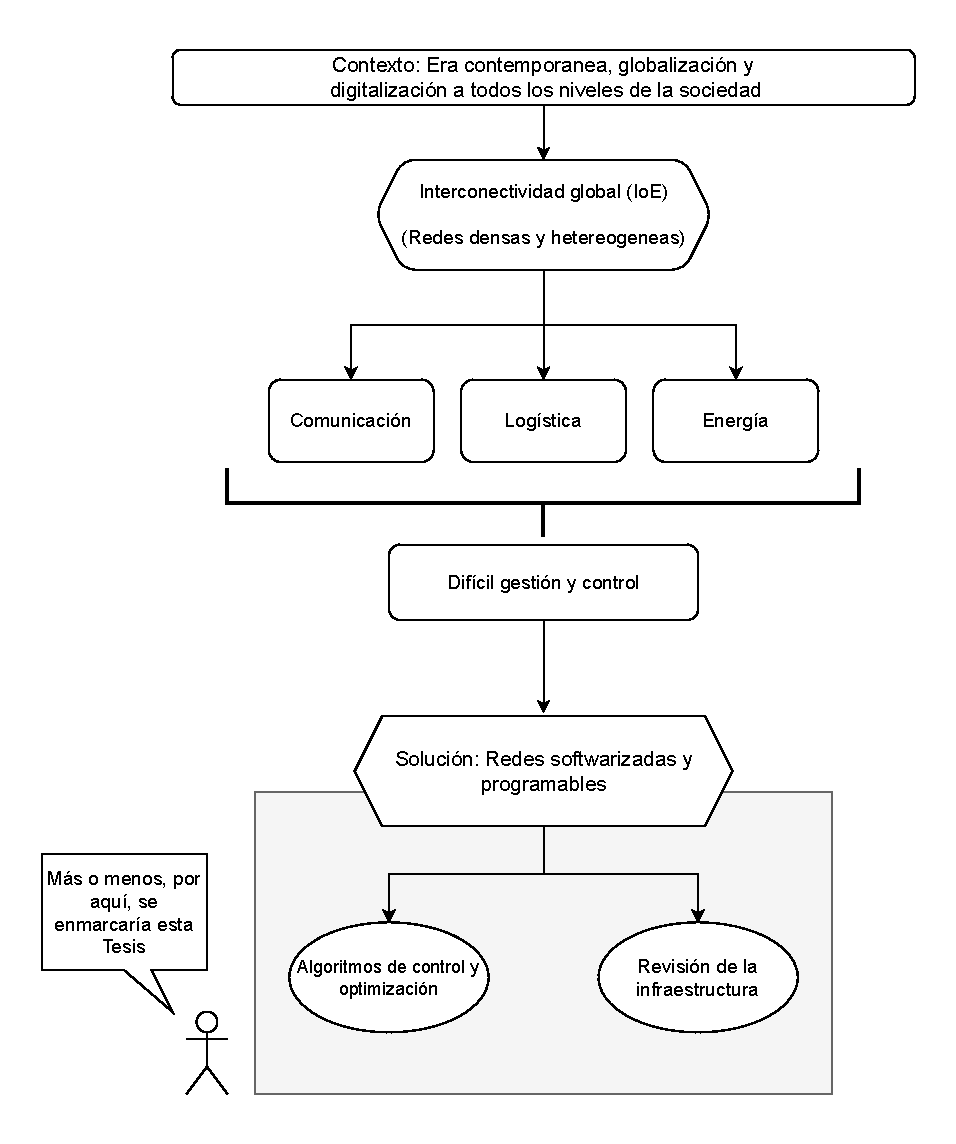
\includegraphics[width=0.85\textwidth]{fig/01_intro/intro_1.drawio.pdf}
    \caption{Diagrama general del marco general de la Tesis}
    \label{fig:intro_1}
\end{figure}

\section{Estructura de la tesis}

A continuación, se presenta la estructura general de esta memoria, describiendo brevemente el contenido de cada uno de sus capítulos. El objetivo es ofrecer una visión global del desarrollo de la Tesis, que sirva como guía para el lector y facilite la comprensión del marco completo del trabajo realizado.\\
\\
El primer capítulo ha contextualizado el ámbito de las redes programables y softwarizadas, destacando su relevancia como base tecnológica para la gestión flexible y dinámica de redes heterogéneas. Asimismo, se ha introducido la problemática asociada a la creciente complejidad de las redes actuales, tanto en las redes de comunicaciones, como las de sensores o las redes de distribución energética, y se han formulado los objetivos principales que guían el desarrollo de esta Tesis. Finalmente, el capítulo concluye con una recopilación de las principales contribuciones científicas generadas a lo largo del trabajo.\\
\\
El segundo capítulo se repasan los conceptos fundamentales y el estado del arte que sustentan la Tesis. El capítulo queda organizado en tres bloques principales. En el primero se abordan las redes programables y softwarizadas, partiendo del paradigma \gls{sdn}, describiendo los modelos de control \textit{out-of-band} e \textit{in-band} y realizando un análisis detallado de las propuestas más relevantes en \textit{in-band}. El segundo bloque se dedica a los servicios y tecnologías habilitadoras en redes softwarizadas y heterogéneas bajo la óptica del MCC (del inglés, Management–Control Continuum): aquí se examinan tanto los servicios básicos (arranque, descubrimiento y provisión de canales de control) como los servicios avanzados (gestión y planificación de recursos, optimización y reconfiguración proactiva de la red). Finalmente, el tercer bloque estudia casos de uso representativos en entornos densos y heterogéneos, con especial atención a las \gls{sg} y a las arquitecturas de sensores \gls{iiot}, para mostrar cómo las tecnologías revisadas se aplican y adaptan a escenarios reales.\\
\\
El tercer capítulo se sintetizan y consolidan los huecos identificados en el capítulo de Estado del Arte, con el objetivo de transformar las lecciones aprendidas en un planteamiento claro del problema, y marcar una hoja de ruta clara para la Tesis.\\
\\
En el capitulo X, .....\\
\\
Por último, el capítulo X recoge las conclusiones principales de la Tesis, así como un bloque que describe futuras líneas de investigación en las que se podrá seguir indagando.


\section{Contribuciones}

El trabajo desarrollado en esta Tesis Doctoral ha generado una contribución notable a la comunidad científica, tanto en términos de generación de conocimiento como en su difusión y transferencia. En concreto, se han publicado cuatro artículos en revistas indexadas en JCR, incluyendo una publicación en una revista de alto impacto Q1 y tres en Q2, y otra dos más que está en revisión (Q2). Además, se han presentado cuatro trabajos en conferencias internacionales organizadas por el IEEE, lo que demuestra la solidez y el interés internacional del trabajo. Como parte del compromiso con la divulgación científica, los avances de esta Tesis también han sido compartidos en eventos como las X Jornadas de Jóvenes Investigadores de la Universidad de Alcalá y la 5th EUGLOH Annual Student Research Conference 2024. Cabe destacar, como elemento diferenciador, el reconocimiento al potencial de transferencia tecnológica de los resultados de esta investigación, materializado en la obtención del Primer Premio en el Concurso de Ideas para la Creación de Empresas de Base Tecnológica de la UAH en 2024. Este premio pone de relieve la capacidad de esta Tesis no solo para generar conocimiento científico de calidad, sino también para transformarlo en soluciones con impacto real en la sociedad, alineadas con los principios de innovación y transferencia del sistema universitario.\\
\\
Artículos de revista indexadas de alto impacto :

\begin{enumerate}
    \item Carrascal, D., Rojas, E., Arco, J. M., Lopez-Pajares, D., Alvarez-Horcajo, J., \& Carral, J. A. (2023). A comprehensive survey of in-band control in sdn: Challenges and opportunities. Electronics, 12(6), 1265. (JCR Q2)
    
    \item Rojas, E., Carrascal, D., Lopez-Pajares, D., Alvarez-Horcajo, J., Carral, J. A., Arco, J. M., \& Martinez-Yelmo, I. (2024). A Survey on AI-Empowered Softwarized Industrial IoT Networks. Electronics, 13(10), 1979. (JCR Q2)
    
    \item Carrascal, D., Rojas, E., Carral, J. A., Martinez-Yelmo, I., \& Alvarez-Horcajo, J. (2024). Topology-aware scalable resource management in multi-hop dense networks. Heliyon, 10(18). (JCR Q1)
    
    \item Carrascal, D., Bartolomé, P., Rojas, E., Lopez-Pajares, D., Manso, N., \& Diaz-Fuentes, J. (2024). Fault Prediction and Reconfiguration Optimization in Smart Grids: AI-Driven Approach. Future Internet, 16(11), 428. (JCR Q2)
    
    \item Carrascal, D., Santos, C., Rojas, E., Arco, J. M., Lopez-Pajares, D. \& Rodriguez-Sanchez F. J. (2025). Dynamic Energy Routing Using Tree-Based Topologies with Fast Convergence applied to Meshed Microgrids. IEEE Access (under review). (JCR Q2)

    \item Carrascal, D., Díaz-Fuentes, J., Manso, N., Lopez-Pajares, D., Rojas, E., Savi, M. \& Arco, J. M. (2025). Softwarized Edge Intelligence for Advanced IIoT Ecosystems: A Data-Driven Architecture Across the Cloud/Edge Continuum. Applied Sciences (under review). (JCR Q2)
  
\end{enumerate}

Conferencias internacionales:

\begin{enumerate}
    \item Carrascal, D., Rojas, E., Lopez-Pajares, D., Manso, N., \& Gutierrez, E. (2023, December). A scalable SDN in-band control protocol for IoT networks in 6G environments. In 2023 6th International Conference on Advanced Communication Technologies and Networking (CommNet) (pp. 1-7). IEEE.
    
    \item Rojas, E., Carrascal, D., Lopez-Pajares, D., Manso, N., \& Arco, J. M. (2024, February). Towards ai-enabled cloud continuum for iiot: Challenges and opportunities. In 2024 International Conference on Artificial Intelligence, Computer, Data Sciences and Applications (ACDSA) (pp. 1-6). IEEE.
    
    \item Comeron, R., Rojas, E., Carrascal, D., Alvarez-Horcajo, J., \& Arco, J. M. (2024, October). Multi-hop collaborative edge computing involving constrained IoT devices at the far edge. In 2024 15th International Conference on Network of the Future (NoF) (pp. 22-24). IEEE.
 
    \item Carrascal, D., Rojas, E., Lopez-Pajares, D., Manso, N., Alvarez-Horcajo, J., \& Martinez-Yelmo, I. (2025, March). Softwarized Data-Driven Architecture for Edge Computing IIoT Environments: A Proof of Concept. In 2025 28th Conference on Innovation in Clouds, Internet and Networks (ICIN) (pp. 64-68). IEEE.
    
\end{enumerate}

Actvidades de divulgación:

\begin{enumerate}
    \item Ponentes a las X Jornadas de Jóvenes Investigadores de la UAH, presentando el trabajo titulado ``DEN2NE: origen, presente, ¿y futuro?''.
    
    \item Participación en la 5th EUGLOH Annual Student Research Conference 2024, con el trabajo titulado ``Advancements in Enabling Technologies for Programmable and Software-Defined Networks: Paving the Way to 6G''.
\end{enumerate}

Premios:

\begin{enumerate}
    \item Primer Premio - Concurso de ideas para la creación de empresas de base tecnológica - UAH (Programa propio de investigación y transferencia de la UAH 2024).
\end{enumerate}

% \begin{figure}[ht]
% \centering
% \resizebox{\textwidth}{!}{%
% \begin{tikzpicture}[
%   font=\small,
%   node distance=1.2cm,
%   milestone/.style={rectangle, draw, rounded corners, fill=blue!10, text width=6cm, align=left},
%   conf/.style={rectangle, draw, rounded corners, fill=green!20, text width=6cm, align=left},
%   year/.style={circle, draw, fill=black!10, minimum size=1cm},
%   line/.style={-{Stealth}, thick}
% ]

% % Año 2023
% \node[year] (y2023) {2023};
% \node[milestone, below=of y2023] (j1) {Electronics 12(6):\\ In-band control in SDN (JCR Q2)};
% \node[conf, below=of j1] (c1) {CommNet 2023:\\ Scalable in-band protocol for IoT};

% % Año 2024
% \node[year, right=6.5cm of y2023] (y2024) {2024};
% \node[milestone, below=of y2024] (j2) {Electronics 13(10):\\ AI for Softwarized IIoT (JCR Q2)};
% \node[milestone, below=of j2] (j3) {Heliyon 10(18):\\ Topology-aware resource mgmt (JCR Q1)};
% \node[milestone, below=of j3] (j4) {Future Internet 16(11):\\ Smart Grid fault prediction (JCR Q2)};
% \node[conf, below=of j4] (c2) {ACDSA 2024:\\ Cloud continuum for IIoT};
% \node[conf, below=of c2] (c3) {NoF 2024:\\ Multi-hop edge computing};

% % Año 2025
% \node[year, right=6.5cm of y2024] (y2025) {2025};
% \node[milestone, below=of y2025] (j5) {IEEE Access (under review):\\ Dynamic energy routing (JCR Q2)};
% \node[conf, below=of j5] (c4) {ICIN 2025:\\ Data-driven edge architecture};

% % Flechas desde año a nodos
% \draw[line] (y2023.south) -- (j1.north);
% \draw[line] (j1.south) -- (c1.north);

% \draw[line] (y2024.south) -- (j2.north);
% \draw[line] (y2024.south) -- (j3.north);
% \draw[line] (y2024.south) -- (j4.north);
% \draw[line] (y2024.south) -- (c2.north);
% \draw[line] (y2024.south) -- (c3.north);

% \draw[line] (y2025.south) -- (j5.north);
% \draw[line] (y2025.south) -- (c4.north);

% \end{tikzpicture}%
% }
% \caption{Timeline of scientific contributions (2023–2025): journal publications and international conferences.}
% \label{fig:timeline_papers}
% \end{figure}

\begin{figure}[ht]
\centering
\begin{tikzpicture}[
  font=\small,
  % --- Estilos de los Nodos (ajustados para ser más compactos) ---
  milestone/.style={
    rectangle, 
    draw, 
    rounded corners, 
    fill=blue!10, 
    text width=3.2cm, % Ancho reducido
    align=center,     % Centrado para mejor estética
    minimum height=1.5cm
  },
  conf/.style={
    rectangle, 
    draw, 
    rounded corners, 
    fill=green!20, 
    text width=3.2cm, % Ancho reducido
    align=center,     % Centrado
    minimum height=1.5cm
  },
  year/.style={
    circle, 
    draw, 
    thick,
    fill=white, 
    minimum size=1cm
  },
  line/.style={
    -{Stealth[length=2mm]}, 
    thick,
    draw=black!70
  }
]

% ---- EJE PRINCIPAL DE LA LÍNEA DE TIEMPO ----
\draw[very thick, -{Stealth[length=3mm]}] (-0.5,0) -- (14.5,0);

% ---- AÑO 2023 ----
\node[year] (y2023) at (1,0) {2023};
% Nodos con texto simplificado
\node[milestone, above=0.8cm of y2023] (j1) {Electronics\\(JCR Q2)};
\node[conf, below=0.8cm of y2023] (c1) {CommNet 2023};

% ---- AÑO 2024 ----
\node[year] (y2024) at (7,0) {2024};
% Nodos con texto simplificado y espaciado ajustado
\node[milestone, above left=0.6cm and 0.1cm of y2024] (j3) {Heliyon\\(JCR Q1)};
\node[milestone, above right=0.6cm and 0.1cm of y2024] (j2) {Electronics\\(JCR Q2)};
\node[milestone, above=3cm of y2024] (j4) {Future Internet\\(JCR Q2)};

\node[conf, below left=0.6cm and 0.1cm of y2024] (c2) {ACDSA 2024};
\node[conf, below right=0.6cm and 0.1cm of y2024] (c3) {NoF 2024};


% ---- AÑO 2025 ----
\node[year] (y2025) at (13,0) {2025};
% Nodos con texto simplificado
% Dado que hoy es 12 de junio de 2025, el estado "under review" es muy relevante.
\node[milestone, above=0.8cm of y2025] (j5) {IEEE Access \& Applied Sciences\\(JCR Q2)\\ (under review)};
\node[conf, below=0.8cm of y2025] (c4) {ICIN 2025};

% ---- CONEXIONES A LA LÍNEA DE TIEMPO ----
% Conexiones 2023
\draw[line] (y2023) -- (j1.south);
\draw[line] (y2023) -- (c1.north);

% Conexiones 2024
\draw[line] (y2024) -- (j2.south);
\draw[line] (y2024) -- (j3.south);
\draw[line] (y2024.north) .. controls +(0,0.8) and +(0,-0.8) .. (j4.south);
\draw[line] (y2024) -- (c2.north);
\draw[line] (y2024) -- (c3.north);

% Conexiones 2025
\draw[line] (y2025) -- (j5.south);
\draw[line] (y2025) -- (c4.north);


\end{tikzpicture}
\caption{Línea de tiempo de contribuciones científicas (2023–2025): publicaciones en revistas y conferencias internacionales.}
\label{fig:timeline_papers_v3}
\end{figure}
\chapter{Estado del Arte}
\label{ch:sota}

Este capítulo tiene como objetivo principal revisar los conceptos clave y el estado del arte que constituyen la base de esta tesis. Para ello, se ha estructurado el capítulo en tres grandes bloques. En primer lugar, se explorarán las redes programables y softwarizadas partiendo de las redes \gls{sdn}, se seguirá con los algoritmos de red y el uso de la \gls{ai} como tecnologías habilitadoras, y por último, se analizarán diversos casos de uso relevantes que ejemplifican la aplicación práctica de estas tecnologías, como son las \gls{sg} y las redes de sensores \gls{iiot}. 

\section{Las redes \glsentryshort{sdn}}
\label{sec:redes_sdn} 

En este primer bloque se revisan las redes \gls{sdn}, que son la base de las redes programables y softwarizadas. Se explorarán sus características, ventajas y desventajas, así como sus paradigmas de modos de control, según se indicó anteriormente. Además, se analizarán los protocolos y así como los aspectos clave de las vertientes de trabajo del modo de control \textit{in-band}, y cómo podemos explorar dicho modo para favorecer la flexibilidad y control en redes densas y heterogéneas.\\
\\
Las redes definidas por software (\gls{sdn}) representan un nuevo paradigma que rompe con las arquitecturas tradicionales de red. Antes de que apareciera el concepto de \gls{sdn}, como se puede apreciar en la Figura~\ref{fig:sdn_paradigma}, las redes tradicionales solían tener un plano de control unificado en los propios dispositivos, llamado generalmente \textit{Control plane}, en el que se definía la lógica que dictaba cómo se debía llevar a cabo el forwarding de los paquetes, y un plano de datos, conocido como \textit{Data plane}, que se implementaba definiendo su datapath, compuesto por varios bloques de procesamiento para reenviar los paquetes. Ambos planos estarían unificados en un sentido lógico, en un mismo dispositivo. Sin embargo, con la aparición del paradigma de las redes \gls{sdn}, como se muestra en la Figura, los nodos tradicionales de la red verían cómo su plano de control sería delegado a una entidad externa llamada controlador, preserbando su capadicar para manejar los paquetes. En contratste con las arquitecturas tradicionales de la red, donde había que ir configurando equipo a equipo, y donde cada uno de ellos iba a desempeñar una función de red, en las redes \gls{sdn}, el controlador permite configurar y supervisar de manera inteligente el comportamiento de la red a través de aplicaciones software, facilitando una programación flexible y dinámica del entorno de red. Por lo que, aunque se sigan llamando ``switches'' o nodos \gls{sdn}, estos se comportarán según las reglas que le instale el controlador, pudiendo gestionar paquetes como un switch, un router, un firewall, etc. 

\begin{figure}[ht!]
\centering
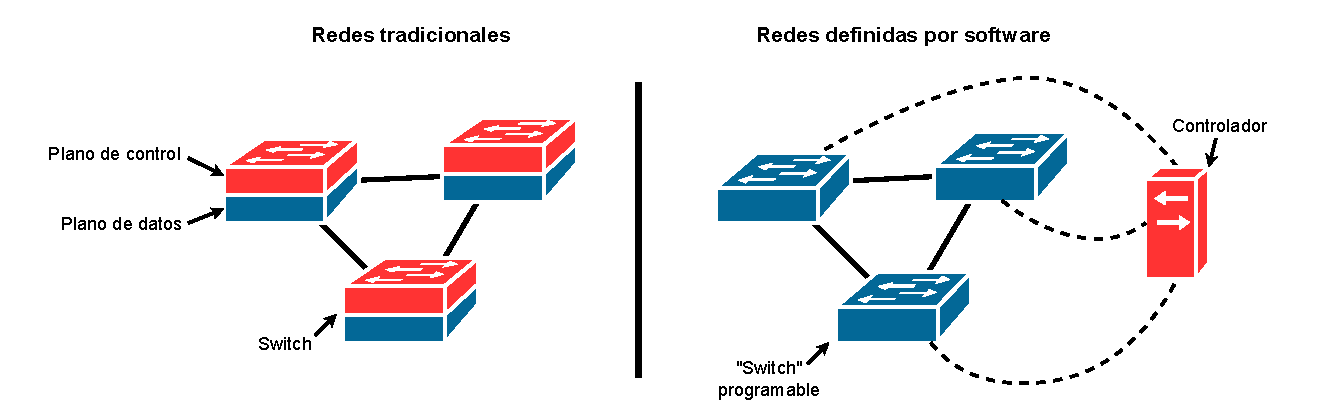
\includegraphics[width=\textwidth]{fig/02_sota/sota_1_sdn_idea.drawio.pdf}
\caption{Paradigma en las redes \glsentryshort{sdn}}
\label{fig:sdn_paradigma}
\end{figure}

La centralización de la gestión simplifica notablemente las tareas del administrador, al proporcionar una visión global del estado de la red y un punto único desde el cual definir su funcionamiento. A través del controlador, las complejas instrucciones de bajo nivel requeridas por los dispositivos de red tradicionales, como switches y routers, las cuales podían variar en función del fabricante, se abstraen mediante interfaces con sintaxis intuitiva, reduciendo la complejidad operativa. Estas capacidades dotan a la red de una gran agilidad y capacidad de adaptación ante cambios o nuevas necesidades, pudiendo conmutar entre distintos perfiles de funcionamiento de forma automática. El simple despliegue de una nueva aplicación sobre el controlador permite modificar de forma coherente el comportamiento de toda la infraestructura, disminuyendo así los costes asociados al mantenimiento, la operación y el despliegue. Además, SDN promueve activamente el uso de soluciones abiertas tanto a nivel de software como de hardware, fomentando ecosistemas interoperables, reduciendo la dependencia de tecnologías propietarias y eliminando barreras de entrada para nuevos actores en el sector.

\subsection{Arquitectura lógica de las redes \glsentryshort{sdn}}
\label{subsec:arquitectura_sdn}

La arquitectura lógica de las redes \gls{sdn} se puede dividir en dos planos, el plano de control y el plano de datos, y además, en tres capas: capa de aplicación, capa de control y capa de infraestructura. En la Figura~\ref{fig:sdn_architecture} se muestra la arquitectura lógica de las redes \gls{sdn}, así como sus interfaces principales de comunicación que más adelante se explicarán.\\
\\
El plano de control, se estructura internamente en dos capas funcionales: la capa de control y la capa de aplicación. Estas se comunican mediante la interfaz norte (northbound interface), que permite a las aplicaciones definir políticas de alto nivel que serán interpretadas y gestionadas por el controlador. Estas capas a menudo se pueden encontrar corriendo en la misma máquina, donde conviven el controlador y las aplicaciones que interactúan con él. Sin embargo, también se puede tener un enfoque distribuido, donde el controlador está en una, máquina, y las aplicaciones en otra, haciendo uso de la interfaz northbound. Por su parte, el plano de datos está conformado por la capa de infraestructura, que engloba los dispositivos físicos de red, principalmente switches \gls{sdn}, responsables del reenvío de paquetes. La interacción entre el plano de control y el plano de datos se realiza a través de la interfaz sur (southbound interface), cuya función es traducir las decisiones del plano de control en instrucciones ejecutables por los dispositivos de red. En este contexto, el controlador actúa como una pieza clave del sistema, asumiendo responsabilidades esenciales como la instalación de reglas de encaminamiento, la monitorización continua del estado de la red y la recopilación de métricas operativas, las cuales serán aprovechadas por todas las aplicaciones que se ejecuten sobre el controlador.

\begin{figure}[ht!]
\centering
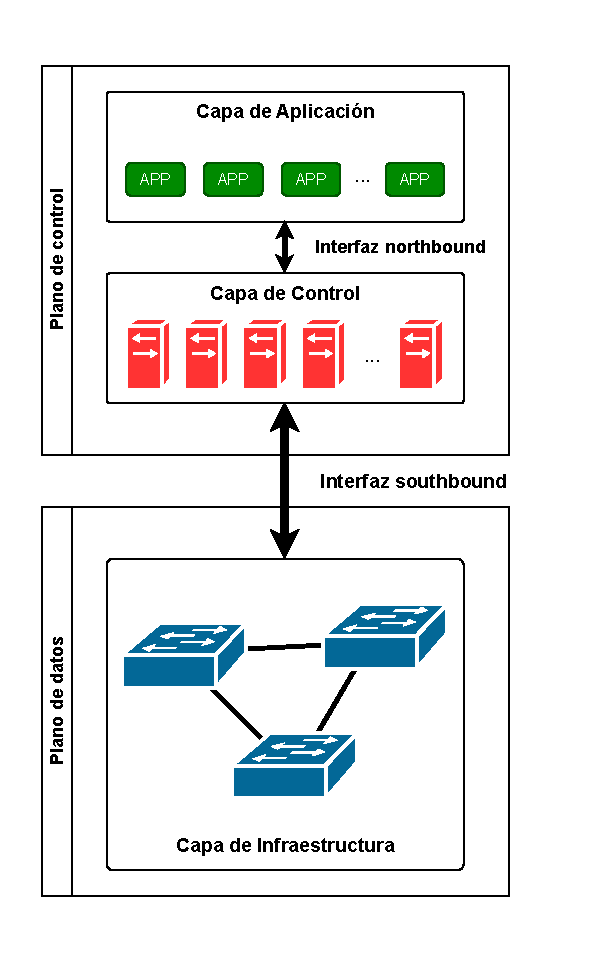
\includegraphics[width=0.5\textwidth]{fig/02_sota/sota_2_sdn_arch_b.drawio.pdf}
\caption{Arquitectura lógica de las redes \glsentryshort{sdn}}
\label{fig:sdn_architecture}
\end{figure}

El plano de datos, por el contrario, no posee lógica de control propia, limitándose a ejecutar las reglas recibidas, como por ejemplo, hacer un reenvío, o descartar paquetes según las reglas establecidas, además de  enviar estadísticas de tráfico al controlador. Esta separación de funciones establece una división clara entre la inteligencia de la red, localizada en el plano de control, y su ejecución, delegada como se ha explicado, al plano de datos. De esta manera, se rompe con el modelo tradicional en el que ambos planos coexistían en un mismo dispositivo de red. Este enfoque modular no solo mejora la escalabilidad y la flexibilidad del sistema, sino que también reduce significativamente los costes de despliegue (\gls{capex}) y operación (\gls{opex}), al concentrar los recursos de cómputo en un nodo centralizado, y simplificar el hardware requerido en los dispositivos de reenvío.\\
\\
Según se ha visto en la Figura~\ref{fig:sdn_architecture}, la arquitectura \gls{sdn} se apoya en una estructura jerárquica formada por tres capas principales: aplicación, control e infraestructura. La capa de aplicación representa el nivel de mayor abstracción dentro del ecosistema \gls{sdn}. Esta capa integra un conjunto de aplicaciones que, apoyándose en los servicios ofrecidos por la capa de control, permiten definir políticas de gestión, \gls{qos}, optimizar el rendimiento de la red y adaptarla dinámicamente a diferentes contextos operativos. Un ejemplo típico de uso es la utilización los servicios de descubrimiento topológico proporcionados por la capa de control, que permiten a las aplicaciones calcular rutas óptimas entre dispositivos de red. Estas aplicaciones suelen desarrollarse empleando lenguajes de alto nivel como Python, Go o C++, con el objetivo de facilitar su portabilidad entre plataformas y maximizar la reutilización del código. No obstante, en la práctica, la existencia de \glspl{api} y entornos de desarrollo específicos para cada plataforma de control, como ONOS, OpenDaylight, Ryu o el nuevo controlador del ecosistema \gls{sdn}, TeraflowSDN, introduce ciertos desafíos en la interoperabilidad y portabilidad del software entre distintas implementaciones. En este sentido, uno de los principales retos actuales de \gls{sdn} sigue siendo la estandarización de interfaces northbound que permitan una integración más fluida y flexible entre aplicaciones y controladores heterogéneos.\\
\\
Descendiendo, la siguiente capa es la capa de control, la cual constituye el núcleo funcional del paradigma \gls{sdn}, albergando la inteligencia centralizada de la red. Actúa como intermediario entre las aplicaciones de alto nivel y los dispositivos físicos de la capa de infraestructura, orquestando tareas críticas como el encaminamiento de flujos, la detección y resolución de fallos, la supervisión continua del estado de la red y la gestión de políticas de seguridad y \gls{qos}. Su papel como middleware se traduce en la capacidad de transformar políticas abstractas generadas en la capa de aplicación en instrucciones simples y concretas que pueden ser entendidas por los nodos \gls{sdn}. Esta capacidad de traducir y escalar la lógica de red permite que un único controlador gobierne cientos o miles de switches de forma eficiente, garantizando escalabilidad y consistencia en entornos distribuidos. Por último, la capa de infraestructura, por su parte, está compuesta por los elementos físicos de la red, fundamentalmente nodos \gls{sdn}, que ejecutan las decisiones tomadas por el plano de control. Estos dispositivos, carentes de lógica propia, cuentan con un agente \gls{sdn} encargado de comunicarse con el controlador a través de la interfaz sur (southbound interface), como por ejemplo, OpenFlow o P4Runtime. Su funcionalidad se reduce al reenvío y descarte de paquetes o la recolección de estadísticas, lo que permite simplificar su diseño y reducir sus requisitos hardware.\\
\\
En cuanto a las interfaces, hay dos, como se ha mencionado anteriormente, la interfaz northbound y la interfaz southbound. La interfaz northbound constituye el canal de comunicación entre la capa de control y la capa de aplicación. Su principal función es ofrecer un punto de acceso lógico al administrador de red, permitiéndole supervisar, configurar y gestionar el comportamiento de la red sin necesidad de interactuar directamente con los mecanismos de bajo nivel que gobiernan los dispositivos físicos. A través de esta interfaz, las aplicaciones pueden programar políticas o solicitudes que serán traducidas por el controlador en instrucciones comprensibles para los elementos de la infraestructura. No obstante, a diferencia de la interfaz southbound, la interfaz northbound carece de una estandarización formal. En consecuencia, la naturaleza y funcionalidad de esta interfaz varían considerablemente en función del controlador \gls{sdn} empleado, cada uno de los cuales suele ofrecer su propia \gls{api} con diferentes modelos de datos, protocolos y lenguajes de interacción.\\
\\
La interfaz southbound constituye el enlace entre la capa de control y la capa de infraestructura dentro de una arquitectura \gls{sdn}. A diferencia de la interfaz northbound, esta sí cuenta con protocolos estandarizados ampliamente adoptados, que permiten la interoperabilidad entre los controladores y los dispositivos de red. Históricamente, el protocolo más representativo ha sido Openflow~\cite{mckeown2008openflow}. En la implementación del protocolo Openflow según se indica en la Figura~\ref{fig:sdn_openflow}, el concepto central es el de flujo (del inglés, \textit{flow}), entendido como un conjunto de paquetes que cumplen determinadas condiciones definidas por el controlador. Estas condiciones se almacenan en las denominadas tablas de flujo (del inglés, \textit{flow tables}), y suelen hacer referencia a valores específicos de campos en la cabecera del paquete o al puerto de entrada por el que se ha recibido.

\begin{figure}[ht!]
\centering
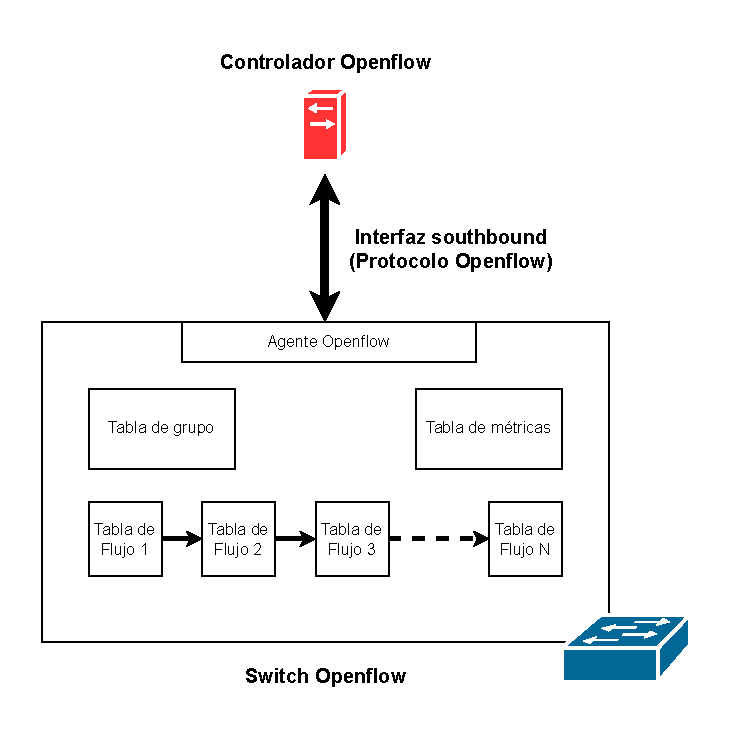
\includegraphics[width=0.7\textwidth]{fig/02_sota/sota_3_sdn_openflow.drawio.pdf}
\caption{Arquitectura básica de switch OpenFlow}
\label{fig:sdn_openflow}
\end{figure}

Cuando un paquete llega a un switch Openflow, empieza a atravesar de forma iterativa las tablas de flujo y cuando este coincide con los criterios de una regla definida en una tabla, se produce una coincidencia (del inglés, \textit{match}), lo que activa un conjunto de instrucciones asociadas a dicha regla. Estas instrucciones pueden incluir el conteo de paquetes, la aplicación de acciones concretas (como reenviar o descartar el paquete), o bien su reenvío hacia otra tabla para un procesamiento adicional. En caso de no darse una coincidencia, se encapsula y se manda al controlador para que este decida que cómo manejarlo. Así, mediante la instalación de estas reglas por parte del controlador \gls{sdn}, se determina el comportamiento de reenvío del switch. La comunicación entre el controlador y los dispositivos se realiza a través de un canal estructurado y seguro, que admite mensajes del controlador al switch, mensajes asíncronos generados por los dispositivos, y mensajes simétricos intercambiables por ambas partes, permitiendo una gestión eficiente y dinámica del estado de red.\\
\\
No obstante, las limitaciones de flexibilidad, extensibilidad y adaptación a nuevas arquitecturas han motivado el surgimiento de alternativas a Openflow. Un ejemplo destacado es el lenguaje \gls{p4}~\cite{bosshart2014p4}, diseñado específicamente para superar las restricciones de OpenFlow. Una de las mayores restricciones que tiene OpenFlow es la especificación de forma explícita de los campos de cabecera sobre los que opera. Estos campos de cabecera han pasado de 12 a 41 campos de cabeceras entre sus versiones 1.0 y 1.5 como se puede ver en la Tabla~\ref{tab:openflow_versions}. Esta evolución ha incrementado la complejidad del protocolo sin proporcionar la flexibilidad necesaria para incorporar nuevas cabeceras o funcionalidades emergentes. 

\begin{table}[ht!]
\centering
\begin{tabular}{|c|c|l|}
\hline
\textbf{Versión} & \textbf{Fecha} & \textbf{Campos de cabecera} \\ \hline
OF 1.0 & Dic. 2009 & 12 campos (Ethernet, TCP/IPv4) \\ \hline
OF 1.1 & Feb. 2011 & 15 campos (MPLS, metadatos entre tablas) \\ \hline
OF 1.2 & Dic. 2011 & 36 campos (ARP, ICMP, IPv6, etc.) \\ \hline
OF 1.3 & Jun. 2012 & 40 campos \\ \hline
OF 1.4 & Oct. 2013 & 41 campos \\ \hline
OF 1.5 & Mar. 2015 & 44 campos \\ \hline
\end{tabular}
\caption{Evolución de versiones del protocolo Openflow y el número de campos de cabecera soportados}    
\label{tab:openflow_versions}
\end{table}

En respuesta a ello, \gls{p4} nació con tres objetivos principales: 

\begin{itemize}
    \item Permitir la reconfiguración del dispositivo en caliente, es decir, cambiar el comportamiento de los switches una vez desplegados.
    
    \item Ofrecer independencia de protocolo, desvinculando el procesamiento de paquetes de protocolos específicos que tengan que estar estandarizados para poder ser gestionados.
    
    \item Proporcionar independencia del hardware, permitiendo que las funcionalidades de procesamiento se definan sin depender de los detalles del dispositivo subyacente. Si bien es cierto que la iniciativa de \gls{p4} nació con este objetivo en mente (\textit{open-hardware}), la realidad es que, en la actualidad, se ha visto como cada fabricante ha implementado equipos que si cumplen con algunas de las arquitecturas de \gls{p4}, pero que cada uno te ofrece unas primitivas de programación diferentes, haciendo que un programa \gls{p4} que corre en un dispositivo de un fabricante no sea totalmente compatible en otro~\cite{hauser2023survey}. 
\end{itemize}

En comparación con Openflow, si nos fijamos en la Figura~\ref{fig:sdn_p4}, podemos apreciar que empleando \gls{p4} se puede definir el cómo el switch va a manejar los paquetes, como los va a procesar y parsear, manteniendo la lógica de las tablas de flujo que teníamos en Openflow, pero ganando en flexibilidad dado que se pueden definir el propio datapath del dispositivo sin depender de un conjunto estandarizado de campos de cabecera. Esto incluso permite que \gls{p4} pueda ser implementado en dispositivos de baja capacidad~\cite{carrascal2020analysis}, al poder ajustar el datapath a la mínima expresión necesaria para cumplir con las necesidades de la red. Al igual que en Openflow se tenía el protocolo de comunicación para la interfaz southbound, \gls{p4} también tiene su propia interfaz de comunicación, llamada P4Runtime~\cite{p4runtime2023}, que permite a los controladores gestionar y programar dispositivos \gls{p4} de forma dinámica. 

\begin{figure}[ht!]
\centering
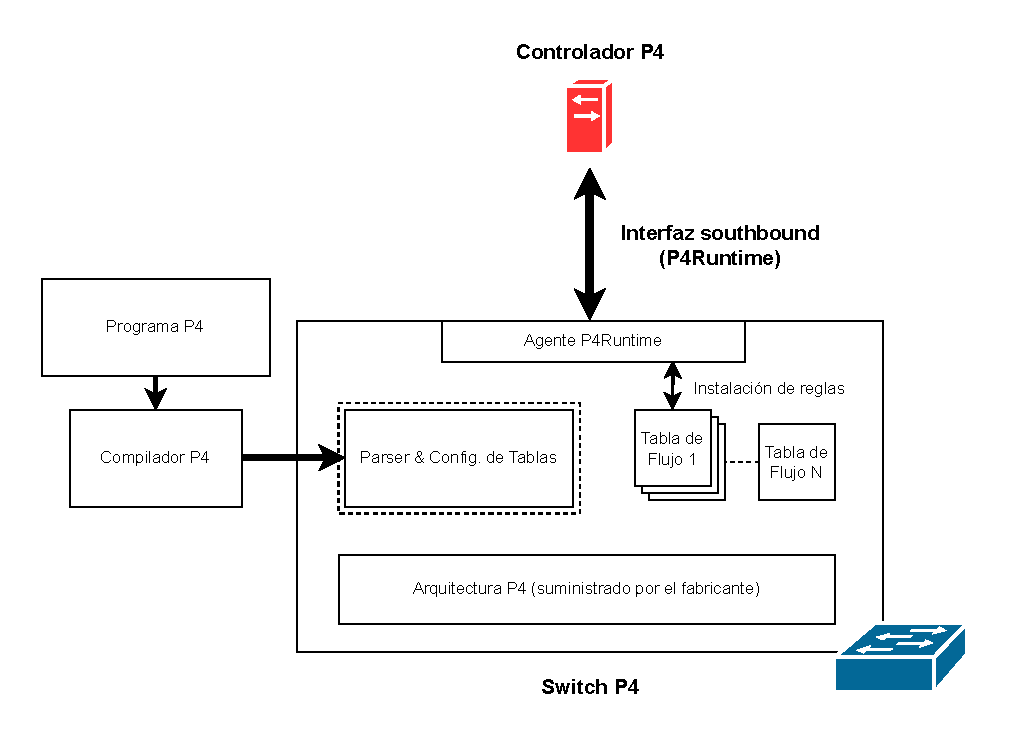
\includegraphics[width=0.9\textwidth]{fig/02_sota/sota_4_sdn_p4.drawio.pdf}
\caption{Arquitectura básica de switch \glsentryshort{p4}}
\label{fig:sdn_p4}
\end{figure}

A diferencia de Openflow, que define un conjunto cerrado de operaciones y estructuras, \gls{p4} y su interfaz P4Runtime introducen la posibilidad de reconfigurar dinámicamente el comportamiento del plano de datos mediante descripciones personalizadas del procesamiento de paquetes. Esto se logra mediante una arquitectura basada en \gls{grpc}, que ofrece cinco tipos de operaciones principales (Write, Read, Set/GetForwardingPipelineConfig y StreamChannel) para gestionar tanto el estado como la lógica interna de los switches programables. De esta forma, \gls{p4} se presenta como una propuesta de evolución de Openflow, orientada a lograr una programabilidad del plano de datos más flexible y escalable, haciéndolo ideal para testing y pruebas de concepto de nuevas soluciones de red.\\
\\
Paralelamente, ha ido creciendo otra vía complementaria orientada a la gestión y configuración unificada de dispositivos de red llamada OpenConfig. Esta iniciativa, impulsada mayormente por un consorcio de operadores y fabricantes, propone un conjunto de modelos de datos basados en YANG que permiten describir de forma estandarizada y agnóstica el estado operativo y la configuración de dispositivos de red. A diferencia de OpenFlow o P4Runtime, que se centran en el comportamiento del plano de reenvío, OpenConfig aborda la gestión, configuración, el monitoreo y la automatización de tareas de red a través de protocolos como gNMI o NETCONF. Esto convierte a OpenConfig una herramienta clave para aquellas empresas que buscan una gestión softwarizada y programable de sus infraestructuras ya existentes, dado que permite la integración de dispositivos heterogéneos de diferentes fabricantes bajo un modelo común de gestión. Si bien es cierto que OpenConfig no permite definir explícitamente el plano de datos, a diferencia de Openflow o \gls{p4}, donde se considera que todos los switches o nodos \gls{sdn} equivalen a un único dispositivo lógico gestionado de forma centralizada, OpenConfig propone un enfoque diferente. Esta iniciativa busca establecer un conjunto común de modelos de datos y configuración, independientes del fabricante, para gestionar redes heterogéneas. A diferencia del enfoque \gls{sdn} tradicional, en el que los dispositivos se integran como un único plano de control y datos, los dispositivos gestionados mediante OpenConfig siguen operando como entidades independientes. Ambos enfoques persiguen una mayor transparencia y facilidad de gestión de la red, pero difieren en su grado de abstracción y centralización: mientras \gls{sdn} trata la red como un todo unificado, OpenConfig mantiene la identidad individual de cada dispositivo, facilitando la interoperabilidad en entornos mixtos. Sin embargo, los últimos controladores \gls{sdn} como TeraflowSDN~\cite{teraflowsdn2021}, han comenzado a integrar OpenConfig como una de sus interfaces southboud (además de \gls{p4}), incluso llegando a no implementar Openflow, lo que sugiere una tendencia hacia un nuevo ecosistema de redes \gls{sdn} que combina la flexibilidad de la programación del plano de datos con la estandarización y la gestión eficiente de dispositivos heterogéneos.\\
\\
En este sentido, la evolución de la interfaz southbound no debe entenderse en términos de sustitución de unos protocolos por otros, sino como una diversificación funcional que permite combinar capacidades de reenvío programable, comunicación eficiente y gestión estandarizada según las necesidades específicas de cada red.


\subsection{Arquitectura física de las redes \glsentryshort{sdn}}
\label{subsec:arquitectura_fisica_sdn}

Una vez que se ha revisado la arquitectura lógica de las redes \gls{sdn}, es importante entender cómo se implementa físicamente esta arquitectura, es decir, cómo se conectan los diferentes componentes que se vienen explicando en la sección anterior.\\
\\
En una red \gls{sdn}, según se indicó en la Figura~\ref{fig:sdn_architecture}, se compone de un elemento central, el controlador, y un conjunto de swicthes o nodos \gls{sdn} distribuidos en la capa de infraestructura los cuales son gestionados por el controlador. Sin embargo, también es posible la implementación de múltiples controladores en una misma red \gls{sdn}, lo cual aporta funcionalidades adicionales a la red, como mecanismos de respaldo y tolerancia a fallos, que incrementan su fiabilidad, y por ende, la resilencia de la red. Por ello, se pueden clasificar las conexiones físicas en las redes \gls{sdn} en dos bloques:  

\begin{itemize}
    \item Las conexiones entre los switches de la capa de infraestructura.
    \item Las conexiones entre el controlador y los switches de la capa de infraestructura.
\end{itemize}
 
Las primeras constituyen la topología física de la red, cuya estructura depende del entorno en el que se despliegue y de los objetivos funcionales de la red. Por ejemplo, en redes \gls{sdn} diseñadas para centros de datos, es común adoptar una arquitectura jerárquica y regular, ya que esta facilita la escalabilidad y permite absorber incrementos en la demanda de tráfico de forma eficiente~\cite{lopez2021nuevos}. En cambio, en entornos de redes de sensores \gls{sdn}, es frecuente emplear topologías en malla parcial (tendiendo hacia a una malla completa)~\cite{baddeley2018evolving}, que permiten una mayor resiliencia frente a fallos y una reducción en la latencia gracias a la existencia de múltiples caminos entre nodos de la topología.\\
\\
En cuanto a las conexiones entre el controlador y los switches de la capa de infraestructura, estas se pueden clasificar en principalmente en dos categorías, si bien es cierto que se puede encontrar una tercera categoría que combina ambas. Observando la Figura~\ref{fig:sdn_control_paradigms}, se pueden distinguir dos paradigmas de control: el modo de control \textit{in-band} y el modo de control \textit{out-of-band}, y por último, el modo de control \textit{hybrid-band}, el cual es una combinación de los dos anteriores. \\

\begin{figure}[ht!]
\centering
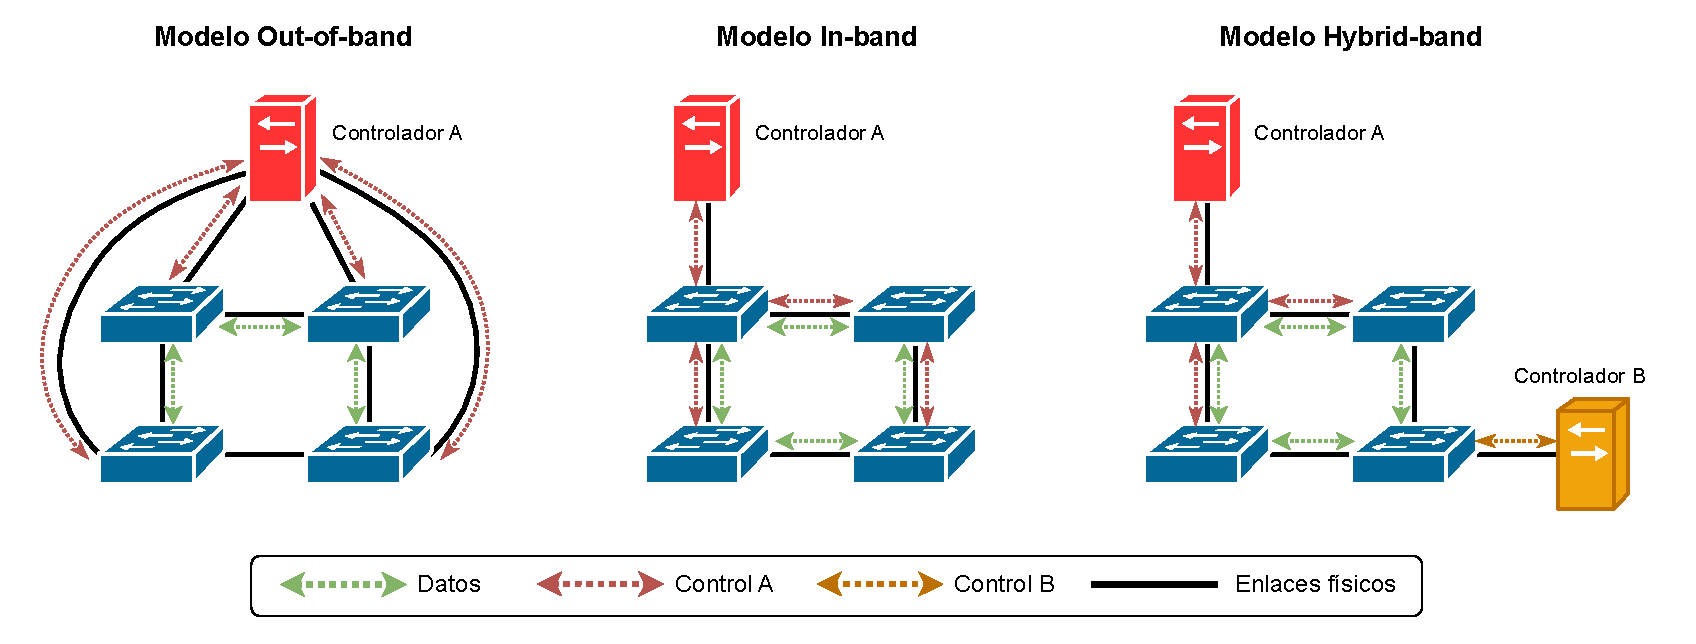
\includegraphics[width=\textwidth]{fig/02_sota/sota_5_sdn_control_paradigms.drawio.pdf}
\caption{Paradigmas de control en las redes \glsentryshort{sdn}}
\label{fig:sdn_control_paradigms}
\end{figure}

Al desplegar el canal de control en una red \gls{sdn}, es posible optar por un enfoque out-of-band o in-band, como se ilustra en la Figura~\ref{fig:sdn_control_paradigms}. En el primer caso, denominado out-of-band, cada nodo \gls{sdn} dispone de un enlace físico dedicado que lo conecta directamente con el controlador. De este modo, la información de control se transmite a través de una red independiente, exclusiva para dicho propósito, lo cual incrementa la seguridad y el aislamiento del canal, aunque implica un mayor coste de infraestructura al requerir al menos un enlace adicional por nodo. Por el contrario, en el enfoque in-band, solo algunos nodos \gls{sdn} mantienen un enlace directo con el controlador, mientras que el resto accede a él a través de la propia red de datos, reutilizando los enlaces existentes para transportar la información de control. En este caso, los mensajes de control comparten la infraestructura del plano de datos, lo que puede comprometer su seguridad e integridad, al estar más expuestos a posibles interferencias o interceptaciones. \\
\\
Finalmente, el enfoque hybrid-band contempla una solución intermedia, en la que coexisten enlaces dedicados y compartidos para la comunicación con el plano de control~\cite{Suo16}, como se muestra en la Figura~\ref{fig:sdn_control_paradigms}. Este modelo busca equilibrar los costes operativos con los requisitos de fiabilidad y seguridad.\\
\\
Cada uno de estos esquemas de despliegue presenta ventajas e inconvenientes~\cite{Suo16}, y la elección entre uno u otro depende fundamentalmente del escenario de red y del caso de uso considerado~\cite{Jalili17,Kafetzis22}. No existe un paradigma mejor que otro, sino, que cada enfoque ofrece características particulares que pueden resultar más o menos adecuadas según los requisitos del entorno. Por ejemplo, el modelo out-of-band requiere un enlace físico adicional dedicado a la comunicación entre el controlador y cada nodo \gls{sdn}, lo que incrementa notablemente los costes de despliegue y mantenimiento. No obstante, esta separación garantiza un mayor aislamiento del canal de control, lo que mejora sustancialmente la seguridad de las comunicaciones. En contraposición, el modelo in-band reutiliza los enlaces existentes del plano de datos para transmitir la información de control, lo que reduce significativamente el coste de infraestructura. Sin embargo, esta economía viene a expensas de una menor seguridad, ya que los mensajes de control comparten canal con el tráfico de red, quedando expuestos a posibles interferencias o ataques. \\
\\
Además, uno de los principales retos del enfoque in-band radica en la configuración inicial, es decir, el nodo debe conocer de antemano la ruta hacia el controlador a través de la red de datos. En contraste, el modelo out-of-band facilita esta tarea, al disponer de una interfaz exclusiva para dicho propósito. Por ello, en in-band, esta información tiene que proporcionarse mediante protocolos específicos que permiten a cada nodo identificar la interfaz adecuada para reenviar los paquetes de control. Estos protocolos son de especial de interés dado que no existe una solución estandarizada en la academia. Debido a lo cual, se quiere explorar en mayor medida qué opciones existen y qué metodologías se han empleado, dado que estas soluciones son fácilmente extrapolables a otros tipos de redes densas y heterogéneas que empleen entornos softwarizados con una tipología de control in-band. Así, por ejemplo, en entornos como el \gls{iot}, donde los dispositivos suelen disponer de una única interfaz de comunicaciones y cuentan con recursos energéticos limitados, el modelo in-band se presenta como una alternativa óptima, al evitar la necesidad de enlaces adicionales que aumentarían el consumo energético y reducirían la vida útil del sensor. \\
\\
La Tabla~\ref{table:inband_adventages} resume comparativamente las principales características de estos modelos. En ella se observa cómo el paradigma out-of-band destaca por su simplicidad de configuración y seguridad, mientras que el in-band sobresale en términos de escalabilidad y costes. 

\begin{table}[ht]
\centering
\resizebox{\textwidth}{!}{%
\begin{tabular}{|l|c|c|}
\hline
\textbf{Propiedad} & \textbf{Control \textit{out-of-band}} & \textbf{Control \textit{in-band}} \\
\hline
Configuración del dispositivo SDN & Sencilla & Compleja \\ \hline
Seguridad del canal de control & Segura, canal aislado & Riesgosa, canal compartido \\ \hline
Costes de mantenimiento y despliegue & Elevados & Reducidos \\ \hline
Escalabilidad & Limitada & Buena \\ \hline
Resiliencia & Costosa & Recuperación rápida\\
\hline
\end{tabular}
}
\caption{Características del control \textit{in-band} y \textit{out-of-band}}
\label{table:inband_adventages}
\end{table}


\subsubsection{Propuestas de despliegue con control in-band}
\label{subsubsec:propuestas_inband}

La tendencia actual indica que el control in-band está ganando protagonismo en los despliegues de redes \gls{sdn}~\cite{Awan19}, especialmente en redes de grandes y densas, donde el coste de utilizar un modelo out-of-band puede resultar prohibitivo. Además, el control in-band habilita el desarrollo de una amplia variedad de nuevas aplicaciones, sobretodo en entornos \gls{sdn} híbridos o con restricciones de recursos~\cite{Khorsandroo21,Rojas21}, donde el despliegue de enlaces dedicados de control puede ser complejo o incluso inviable. Entre los casos de uso más representativos que se benefician del control in-band se encuentran las redes \gls{5g}~\cite{Murtadha21} y las \glspl{ntn}~\cite{Guo21}, así como diversos escenarios del ámbito \gls{iot}, como redes submarinas~\cite{Shi22}, entornos orientados a la eficiencia energética~\cite{Maity22} o sistemas con recursos limitados~\cite{Chattopadhyay19}. A pesar de sus numerosas ventajas, los esfuerzos dirigidos al diseño de protocolos comunes e integrales para el control in-band han sido escasos. Una solución efectiva debería considerar la compatibilidad con plataformas ampliamente utilizadas, tanto en los controladores como en los dispositivos \gls{sdn}, a fin de garantizar una integración completa en los despliegues actuales. En este contexto, diferentes propuestas han explorado mecanismos para habilitar o mejorar el control in-band, con el objetivo de facilitar su adopción en entornos reales y responder a los retos que plantea,este paradigma. A continuación, se presentan algunos de los trabajos más representativos en esta línea.\\
\\
%En este contexto, los trabajos existentes sobre control in-band pueden clasificarse en función de tres aspectos clave que dicho paradigma debería proporcionar: encaminamiento automático, recuperación rápida ante fallos y arranque autónomo de la red. Además, se ha identificado un cuarto aspecto transversal, relacionado con entornos de control distribuido que tambien merece la pena revisar. En primer lugar, la necesidad de contar con un mecanismo de encaminamiento automático en el control in-band resulta evidente. Mientras que el modelo out-of-band suele implementarse mediante enlaces directos entre los nodos \gls{sdn} y el controlador, el control in-band requiere calcular rutas entre los dispositivos de red y uno o varios controladores, tanto en un sentido ascendente, como descendente. Este mecanismo de encaminamiento es esencial para permitir la comunicación de control a través del plano de datos y suele condicionarse al tipo de despliegue o a las capacidades del entorno. En segundo lugar, una de las principales ventajas del control in-band es su capacidad de recuperación rápida ante fallos. En caso de que un enlace o switch sufra una avería, es posible restaurar la comunicación de control simplemente seleccionando una ruta alternativa dentro del plano de datos. No obstante, para que este proceso resulte eficaz, los mecanismos de restauración o protección de rutas deben estar bien definidos y coordinados con la lógica de encaminamiento previamente establecida. El tercer aspecto fundamental es el denominado arranque autónomo de la red (del inglés, \textit{network bootstrapping}), que hace referencia a la capacidad del sistema para configurar automáticamente los parámetros necesarios antes del inicio de su operación. Estos parámetros incluyen, entre otros, la información de conectividad entre nodos \gls{sdn} y controladores. Si bien este proceso también es deseable en entornos out-of-band, en el caso de control in-band se convierte en un requisito crítico, ya que las rutas de control pueden variar en función del despliegue y del protocolo de encaminamiento utilizado. Por último, en entornos con control distribuido, donde existen varios controladores implicados en la toma de decisiones, es necesario incorporar mecanismos de coordinación que permitan compartir rutas, realizar recuperación ante fallos de manera conjunta y gestionar el arranque de la red de forma sincronizada. Además, el control in-band puede ofrecer un canal adicional para la comunicación interna entre controladores, lo cual añade una dimensión interesante a su uso en arquitecturas distribuidas.\\
%\\

%En primer lugar, varios autores han sentado las bases de un marco genérico de control in-band y han explorado mecanismos de recuperación ante fallos simples. Sharma et al.\cite{Sharma16} presentan un prototipo basado en OpenFlow y NOX que evalúa la viabilidad de este paradigma en distintos switches, proponiendo métodos de restauración y protección frente a fallos individuales. De manera similar, Goltsmann et al.\cite{Goltsmann17} introducen el protocolo ICS, que construye un árbol de expansión etiquetado para garantizar conectividad resiliente con bajo sobrecoste. Ambos trabajos ponen de manifiesto la factibilidad del control in-band en escenarios sencillos, pero no extienden sus propuestas a la gestión simultánea de múltiples fallos ni proporcionan un estándar interoperable.

%Un segundo bloque de investigaciones se centra en la tolerancia a múltiples fallos y en la complejidad de su implementación práctica. Khakhalin et al.\cite{Khakhalin17} formulan un algoritmo resistente a múltiples averías mediante la asignación de etiquetas únicas a cada switch, aunque la gestión de estas etiquetas se complica rápidamente en redes de gran escala. Por su parte, Mohan et al.\cite{Mohan18} definen un esquema de rutas de control disjuntas por nodo para detectar y aislar switches maliciosos; si bien mejora la seguridad, su formulación matemática no escala bien debido al elevado número de variables de decisión.

%Un tercer grupo aborda la disponibilidad del canal y el arranque autónomo de la red. Raza et al.\cite{Raza17} y González et al.\cite{Gonzalez18} investigan el uso de \gls{mptcp} para aumentar la tolerancia de rutas, aunque ambos dependen de un enlace out-of-band inicial para la fase de arranque. Fan et al.~\cite{Fan20}, por su parte, diseñan un algoritmo centralizado que ubica el canal in-band en el enlace con mayor ancho de banda disponible, mejorando métricas como RTT y PLR en topologías tipo Fat-Tree; no obstante, su solución no se ha validado en redes genéricas de gran tamaño.

%Finalmente, existen propuestas más avanzadas y específicas para entornos heterogéneos. Görkemli et al.\cite{Gorkemli18} plantean un plano de control dinámico capaz de redistribuir carga entre varios controladores y adaptar el enrutamiento in-band según la topología y las necesidades de las aplicaciones; sin embargo, su evaluación solo contempla despliegues virtualizados. Holzmann et al.\cite{Holzmann19} presentan Izzy, un protocolo distribuido basado en árboles de expansión y direcciones temporales que logra tiempos de recuperación inferiores a 100 ms en simulaciones WAN de 100 nodos, aunque aún no dispone de validación en entornos reales. En el ámbito de redes satelitales, Ningyuan et al.\cite{Ningyuan21} proponen una arquitectura de doble capa para constelaciones \gls{leo}, que garantiza rutas fiables pese a la movilidad de los satélites, si bien su propuesta permanece en fase de simulación. Por último, Kumazoe et al.\cite{Kumazoe22} diseñan un canal in-band en entornos \gls{p4}, embebiendo mensajes de control en paquetes de usuario; aunque innovador, su evaluación inicial revela degradaciones en el reenvío de datos que quedan pendientes de resolver.




\section{Algoritmos de red y \glsentryshort{ai}}
\label{sec:tecnologias_habilitantes}

En este segundo bloque se quieren revisar las principales tecnologías habilitantes que permiten la creeación, control y gestión de las redes programables y softwarizadas. Estas tecnologías son fundamentales para entender el marco de trabajo de la tesis, y cómo, posteriormente, se pueden llegar a aplicar a diferentes casos de uso. 


\section{Casos de uso}  
\label{sec:casos_de_uso}
En este último bloque se revisan los casos de uso más relevantes que se pueden encontrar en la literatura. Estos casos de uso son ejemplos prácticos de cómo las tecnologías habilitantes y las redes programables y softwarizadas se aplican en contextos reales, como las \gls{sg} y las redes de sensores \gls{iiot}. 
\chapter{Capítulo de prueba}
\label{chap:test}

Este capítulo tiene como propósito verificar la correcta configuración de los índices e instrumentos del documento.

\section{Uso de acrónimos y referencias}
En este documento se utiliza el concepto de \gls{sdn}, el cual es fundamental en redes programables. Para más detalles, véase el capítulo de introducción. 

Lorem ipsum dolor sit amet, consectetur adipiscing elit. Vivamus finibus, diam non blandit interdum, eros urna accumsan lectus, in aliquet libero neque in tortor. Quisque condimentum posuere ex, ac bibendum dolor posuere ac. Integer dolor metus, sollicitudin a consequat id, eleifend in magna. Pellentesque sed magna hendrerit, aliquet diam non, mollis massa. Phasellus tempus efficitur eros, quis malesuada felis pulvinar ut. Cras feugiat eget velit ut ultricies. Vivamus a tincidunt ante. Fusce neque tellus, molestie quis augue id, pulvinar maximus sapien. Sed blandit ex quis felis sodales, quis semper libero ultrices. Aenean eros lacus, bibendum at ex auctor, accumsan sagittis mauris.

Ut gravida mauris in velit maximus pellentesque. Praesent ultricies, mi eu convallis laoreet, lorem leo euismod urna, non imperdiet ligula purus vestibulum felis. Nam consequat lorem eget leo dictum, vel viverra enim commodo. Maecenas ac porttitor velit, nec dignissim velit. In tellus massa, ornare id est finibus, mattis tristique velit. Sed vitae interdum lectus. Sed placerat quam sit amet lacus lacinia, nec tristique libero efficitur. Ut varius lobortis velit. Mauris euismod dictum luctus. Aliquam neque quam, vehicula quis mollis eget, sollicitudin id elit. Integer cursus risus ac purus fringilla, facilisis condimentum dui sagittis. Pellentesque gravida turpis dui, nec consequat lacus scelerisque et.

Sed mollis, purus at malesuada mattis, dui sem scelerisque lectus, ut fermentum leo urna eget diam. Duis facilisis turpis nibh, in commodo nisi pretium nec. Donec finibus elit et felis elementum finibus. Donec turpis purus, rutrum sit amet orci eu, tincidunt porta quam. Etiam velit mauris, varius in risus at, sodales consectetur metus. Ut urna turpis, ornare id lectus vitae, ultrices cursus urna. Nunc lacinia ullamcorper nunc in facilisis. Fusce rhoncus eros elit, at posuere ex vulputate vel. Phasellus ullamcorper neque eu ante porttitor, vel iaculis justo lobortis. Vestibulum ornare eros ex, eget porta felis ultrices vitae. Donec mauris arcu, vulputate vel lectus vitae, semper tempus ligula.

Maecenas eros dolor, auctor tincidunt enim in, bibendum ultricies magna. Aenean pellentesque interdum condimentum. Cras sollicitudin vel lorem vitae lacinia. Phasellus pulvinar suscipit volutpat. Sed ac vulputate erat, vel luctus ligula. Curabitur pretium mollis ornare. In sit amet nisl quis eros efficitur mollis. Quisque iaculis nisl sed tincidunt condimentum.

Suspendisse finibus, nunc a ultricies tempor, ex neque scelerisque diam, in varius ligula lectus ut nulla. Suspendisse dapibus mi vitae tellus consequat fermentum. Integer bibendum nisl quam, dignissim egestas augue efficitur vitae. Integer pellentesque felis nisl, id iaculis orci maximus sed. Sed blandit pretium leo, volutpat varius quam vestibulum sed. Curabitur sit amet volutpat eros. Nulla vitae tristique tellus. Duis efficitur nec libero placerat pharetra. Cras luctus neque a lorem mattis, eget laoreet magna pharetra. Nam ipsum ligula, hendrerit a orci vitae, ultricies auctor felis. Vestibulum at elit non tellus dapibus lobortis. Donec quis consectetur nibh, sit amet commodo massa. Sed ultrices, velit sed lacinia congue, ipsum mauris suscipit libero, vel posuere est ipsum eu justo. Aliquam ut venenatis neque, ut volutpat nunc. Suspendisse finibus ornare dolor sit amet tristique. Fusce a porta mauris.

Phasellus egestas augue id purus vestibulum, vel posuere ipsum dictum. Fusce eget bibendum dui. Maecenas tempus, sapien at vulputate pretium, elit felis dignissim velit, sit amet feugiat tellus quam vel turpis. Aenean quis viverra nulla, vel rhoncus augue. Morbi sit amet elit fermentum, finibus justo tristique, ultricies sapien. Sed sit amet lacinia nunc, ac pretium mauris. Donec dapibus velit non nunc sagittis semper. Ut ut nulla volutpat, rhoncus libero at, venenatis lorem. Maecenas iaculis dictum arcu eu accumsan. Donec non metus justo. Praesent non ipsum a nisl venenatis efficitur. Etiam lacinia, elit non tristique tincidunt, sapien erat malesuada diam, sed accumsan augue est eget ante. Maecenas at odio accumsan, luctus sem id, lacinia quam.

Sed at nisi erat. Integer scelerisque erat vitae aliquam sagittis. Duis id ipsum auctor orci dapibus porta vel quis augue. Vivamus consectetur dapibus turpis. Vivamus id facilisis nisi, quis fermentum urna. Ut fringilla auctor faucibus. Ut eu sapien nisi. Cras lorem risus, finibus sed scelerisque vel, commodo pulvinar lacus. In at luctus ante, non commodo quam.
Lorem ipsum dolor sit amet, consectetur adipiscing elit. Vivamus finibus, diam non blandit interdum, eros urna accumsan lectus, in aliquet libero neque in tortor. Quisque condimentum posuere ex, ac bibendum dolor posuere ac. Integer dolor metus, sollicitudin a consequat id, eleifend in magna. Pellentesque sed magna hendrerit, aliquet diam non, mollis massa. Phasellus tempus efficitur eros, quis malesuada felis pulvinar ut. Cras feugiat eget velit ut ultricies. Vivamus a tincidunt ante. Fusce neque tellus, molestie quis augue id, pulvinar maximus sapien. Sed blandit ex quis felis sodales, quis semper libero ultrices. Aenean eros lacus, bibendum at ex auctor, accumsan sagittis mauris.

Ut gravida mauris in velit maximus pellentesque. Praesent ultricies, mi eu convallis laoreet, lorem leo euismod urna, non imperdiet ligula purus vestibulum felis. Nam consequat lorem eget leo dictum, vel viverra enim commodo. Maecenas ac porttitor velit, nec dignissim velit. In tellus massa, ornare id est finibus, mattis tristique velit. Sed vitae interdum lectus. Sed placerat quam sit amet lacus lacinia, nec tristique libero efficitur. Ut varius lobortis velit. Mauris euismod dictum luctus. Aliquam neque quam, vehicula quis mollis eget, sollicitudin id elit. Integer cursus risus ac purus fringilla, facilisis condimentum dui sagittis. Pellentesque gravida turpis dui, nec consequat lacus scelerisque et.

Sed mollis, purus at malesuada mattis, dui sem scelerisque lectus, ut fermentum leo urna eget diam. Duis facilisis turpis nibh, in commodo nisi pretium nec. Donec finibus elit et felis elementum finibus. Donec turpis purus, rutrum sit amet orci eu, tincidunt porta quam. Etiam velit mauris, varius in risus at, sodales consectetur metus. Ut urna turpis, ornare id lectus vitae, ultrices cursus urna. Nunc lacinia ullamcorper nunc in facilisis. Fusce rhoncus eros elit, at posuere ex vulputate vel. Phasellus ullamcorper neque eu ante porttitor, vel iaculis justo lobortis. Vestibulum ornare eros ex, eget porta felis ultrices vitae. Donec mauris arcu, vulputate vel lectus vitae, semper tempus ligula.

Maecenas eros dolor, auctor tincidunt enim in, bibendum ultricies magna. Aenean pellentesque interdum condimentum. Cras sollicitudin vel lorem vitae lacinia. Phasellus pulvinar suscipit volutpat. Sed ac vulputate erat, vel luctus ligula. Curabitur pretium mollis ornare. In sit amet nisl quis eros efficitur mollis. Quisque iaculis nisl sed tincidunt condimentum.

Suspendisse finibus, nunc a ultricies tempor, ex neque scelerisque diam, in varius ligula lectus ut nulla. Suspendisse dapibus mi vitae tellus consequat fermentum. Integer bibendum nisl quam, dignissim egestas augue efficitur vitae. Integer pellentesque felis nisl, id iaculis orci maximus sed. Sed blandit pretium leo, volutpat varius quam vestibulum sed. Curabitur sit amet volutpat eros. Nulla vitae tristique tellus. Duis efficitur nec libero placerat pharetra. Cras luctus neque a lorem mattis, eget laoreet magna pharetra. Nam ipsum ligula, hendrerit a orci vitae, ultricies auctor felis. Vestibulum at elit non tellus dapibus lobortis. Donec quis consectetur nibh, sit amet commodo massa. Sed ultrices, velit sed lacinia congue, ipsum mauris suscipit libero, vel posuere est ipsum eu justo. Aliquam ut venenatis neque, ut volutpat nunc. Suspendisse finibus ornare dolor sit amet tristique. Fusce a porta mauris.

Phasellus egestas augue id purus vestibulum, vel posuere ipsum dictum. Fusce eget bibendum dui. Maecenas tempus, sapien at vulputate pretium, elit felis dignissim velit, sit amet feugiat tellus quam vel turpis. Aenean quis viverra nulla, vel rhoncus augue. Morbi sit amet elit fermentum, finibus justo tristique, ultricies sapien. Sed sit amet lacinia nunc, ac pretium mauris. Donec dapibus velit non nunc sagittis semper. Ut ut nulla volutpat, rhoncus libero at, venenatis lorem. Maecenas iaculis dictum arcu eu accumsan. Donec non metus justo. Praesent non ipsum a nisl venenatis efficitur. Etiam lacinia, elit non tristique tincidunt, sapien erat malesuada diam, sed accumsan augue est eget ante. Maecenas at odio accumsan, luctus sem id, lacinia quam.

Sed at nisi erat. Integer scelerisque erat vitae aliquam sagittis. Duis id ipsum auctor orci dapibus porta vel quis augue. Vivamus consectetur dapibus turpis. Vivamus id facilisis nisi, quis fermentum urna. Ut fringilla auctor faucibus. Ut eu sapien nisi. Cras lorem risus, finibus sed scelerisque vel, commodo pulvinar lacus. In at luctus ante, non commodo quam.
Lorem ipsum dolor sit amet, consectetur adipiscing elit. Vivamus finibus, diam non blandit interdum, eros urna accumsan lectus, in aliquet libero neque in tortor. Quisque condimentum posuere ex, ac bibendum dolor posuere ac. Integer dolor metus, sollicitudin a consequat id, eleifend in magna. Pellentesque sed magna hendrerit, aliquet diam non, mollis massa. Phasellus tempus efficitur eros, quis malesuada felis pulvinar ut. Cras feugiat eget velit ut ultricies. Vivamus a tincidunt ante. Fusce neque tellus, molestie quis augue id, pulvinar maximus sapien. Sed blandit ex quis felis sodales, quis semper libero ultrices. Aenean eros lacus, bibendum at ex auctor, accumsan sagittis mauris.

Ut gravida mauris in velit maximus pellentesque. Praesent ultricies, mi eu convallis laoreet, lorem leo euismod urna, non imperdiet ligula purus vestibulum felis. Nam consequat lorem eget leo dictum, vel viverra enim commodo. Maecenas ac porttitor velit, nec dignissim velit. In tellus massa, ornare id est finibus, mattis tristique velit. Sed vitae interdum lectus. Sed placerat quam sit amet lacus lacinia, nec tristique libero efficitur. Ut varius lobortis velit. Mauris euismod dictum luctus. Aliquam neque quam, vehicula quis mollis eget, sollicitudin id elit. Integer cursus risus ac purus fringilla, facilisis condimentum dui sagittis. Pellentesque gravida turpis dui, nec consequat lacus scelerisque et.

Sed mollis, purus at malesuada mattis, dui sem scelerisque lectus, ut fermentum leo urna eget diam. Duis facilisis turpis nibh, in commodo nisi pretium nec. Donec finibus elit et felis elementum finibus. Donec turpis purus, rutrum sit amet orci eu, tincidunt porta quam. Etiam velit mauris, varius in risus at, sodales consectetur metus. Ut urna turpis, ornare id lectus vitae, ultrices cursus urna. Nunc lacinia ullamcorper nunc in facilisis. Fusce rhoncus eros elit, at posuere ex vulputate vel. Phasellus ullamcorper neque eu ante porttitor, vel iaculis justo lobortis. Vestibulum ornare eros ex, eget porta felis ultrices vitae. Donec mauris arcu, vulputate vel lectus vitae, semper tempus ligula.

Maecenas eros dolor, auctor tincidunt enim in, bibendum ultricies magna. Aenean pellentesque interdum condimentum. Cras sollicitudin vel lorem vitae lacinia. Phasellus pulvinar suscipit volutpat. Sed ac vulputate erat, vel luctus ligula. Curabitur pretium mollis ornare. In sit amet nisl quis eros efficitur mollis. Quisque iaculis nisl sed tincidunt condimentum.

Suspendisse finibus, nunc a ultricies tempor, ex neque scelerisque diam, in varius ligula lectus ut nulla. Suspendisse dapibus mi vitae tellus consequat fermentum. Integer bibendum nisl quam, dignissim egestas augue efficitur vitae. Integer pellentesque felis nisl, id iaculis orci maximus sed. Sed blandit pretium leo, volutpat varius quam vestibulum sed. Curabitur sit amet volutpat eros. Nulla vitae tristique tellus. Duis efficitur nec libero placerat pharetra. Cras luctus neque a lorem mattis, eget laoreet magna pharetra. Nam ipsum ligula, hendrerit a orci vitae, ultricies auctor felis. Vestibulum at elit non tellus dapibus lobortis. Donec quis consectetur nibh, sit amet commodo massa. Sed ultrices, velit sed lacinia congue, ipsum mauris suscipit libero, vel posuere est ipsum eu justo. Aliquam ut venenatis neque, ut volutpat nunc. Suspendisse finibus ornare dolor sit amet tristique. Fusce a porta mauris.

Phasellus egestas augue id purus vestibulum, vel posuere ipsum dictum. Fusce eget bibendum dui. Maecenas tempus, sapien at vulputate pretium, elit felis dignissim velit, sit amet feugiat tellus quam vel turpis. Aenean quis viverra nulla, vel rhoncus augue. Morbi sit amet elit fermentum, finibus justo tristique, ultricies sapien. Sed sit amet lacinia nunc, ac pretium mauris. Donec dapibus velit non nunc sagittis semper. Ut ut nulla volutpat, rhoncus libero at, venenatis lorem. Maecenas iaculis dictum arcu eu accumsan. Donec non metus justo. Praesent non ipsum a nisl venenatis efficitur. Etiam lacinia, elit non tristique tincidunt, sapien erat malesuada diam, sed accumsan augue est eget ante. Maecenas at odio accumsan, luctus sem id, lacinia quam.

Sed at nisi erat. Integer scelerisque erat vitae aliquam sagittis. Duis id ipsum auctor orci dapibus porta vel quis augue. Vivamus consectetur dapibus turpis. Vivamus id facilisis nisi, quis fermentum urna. Ut fringilla auctor faucibus. Ut eu sapien nisi. Cras lorem risus, finibus sed scelerisque vel, commodo pulvinar lacus. In at luctus ante, non commodo quam.

\section{Figura de prueba}

En la Figura~\ref{fig:arquitectura}, se muestra un esquema conceptual básico de una red softwarizada.

\begin{figure}[ht]
    \centering
    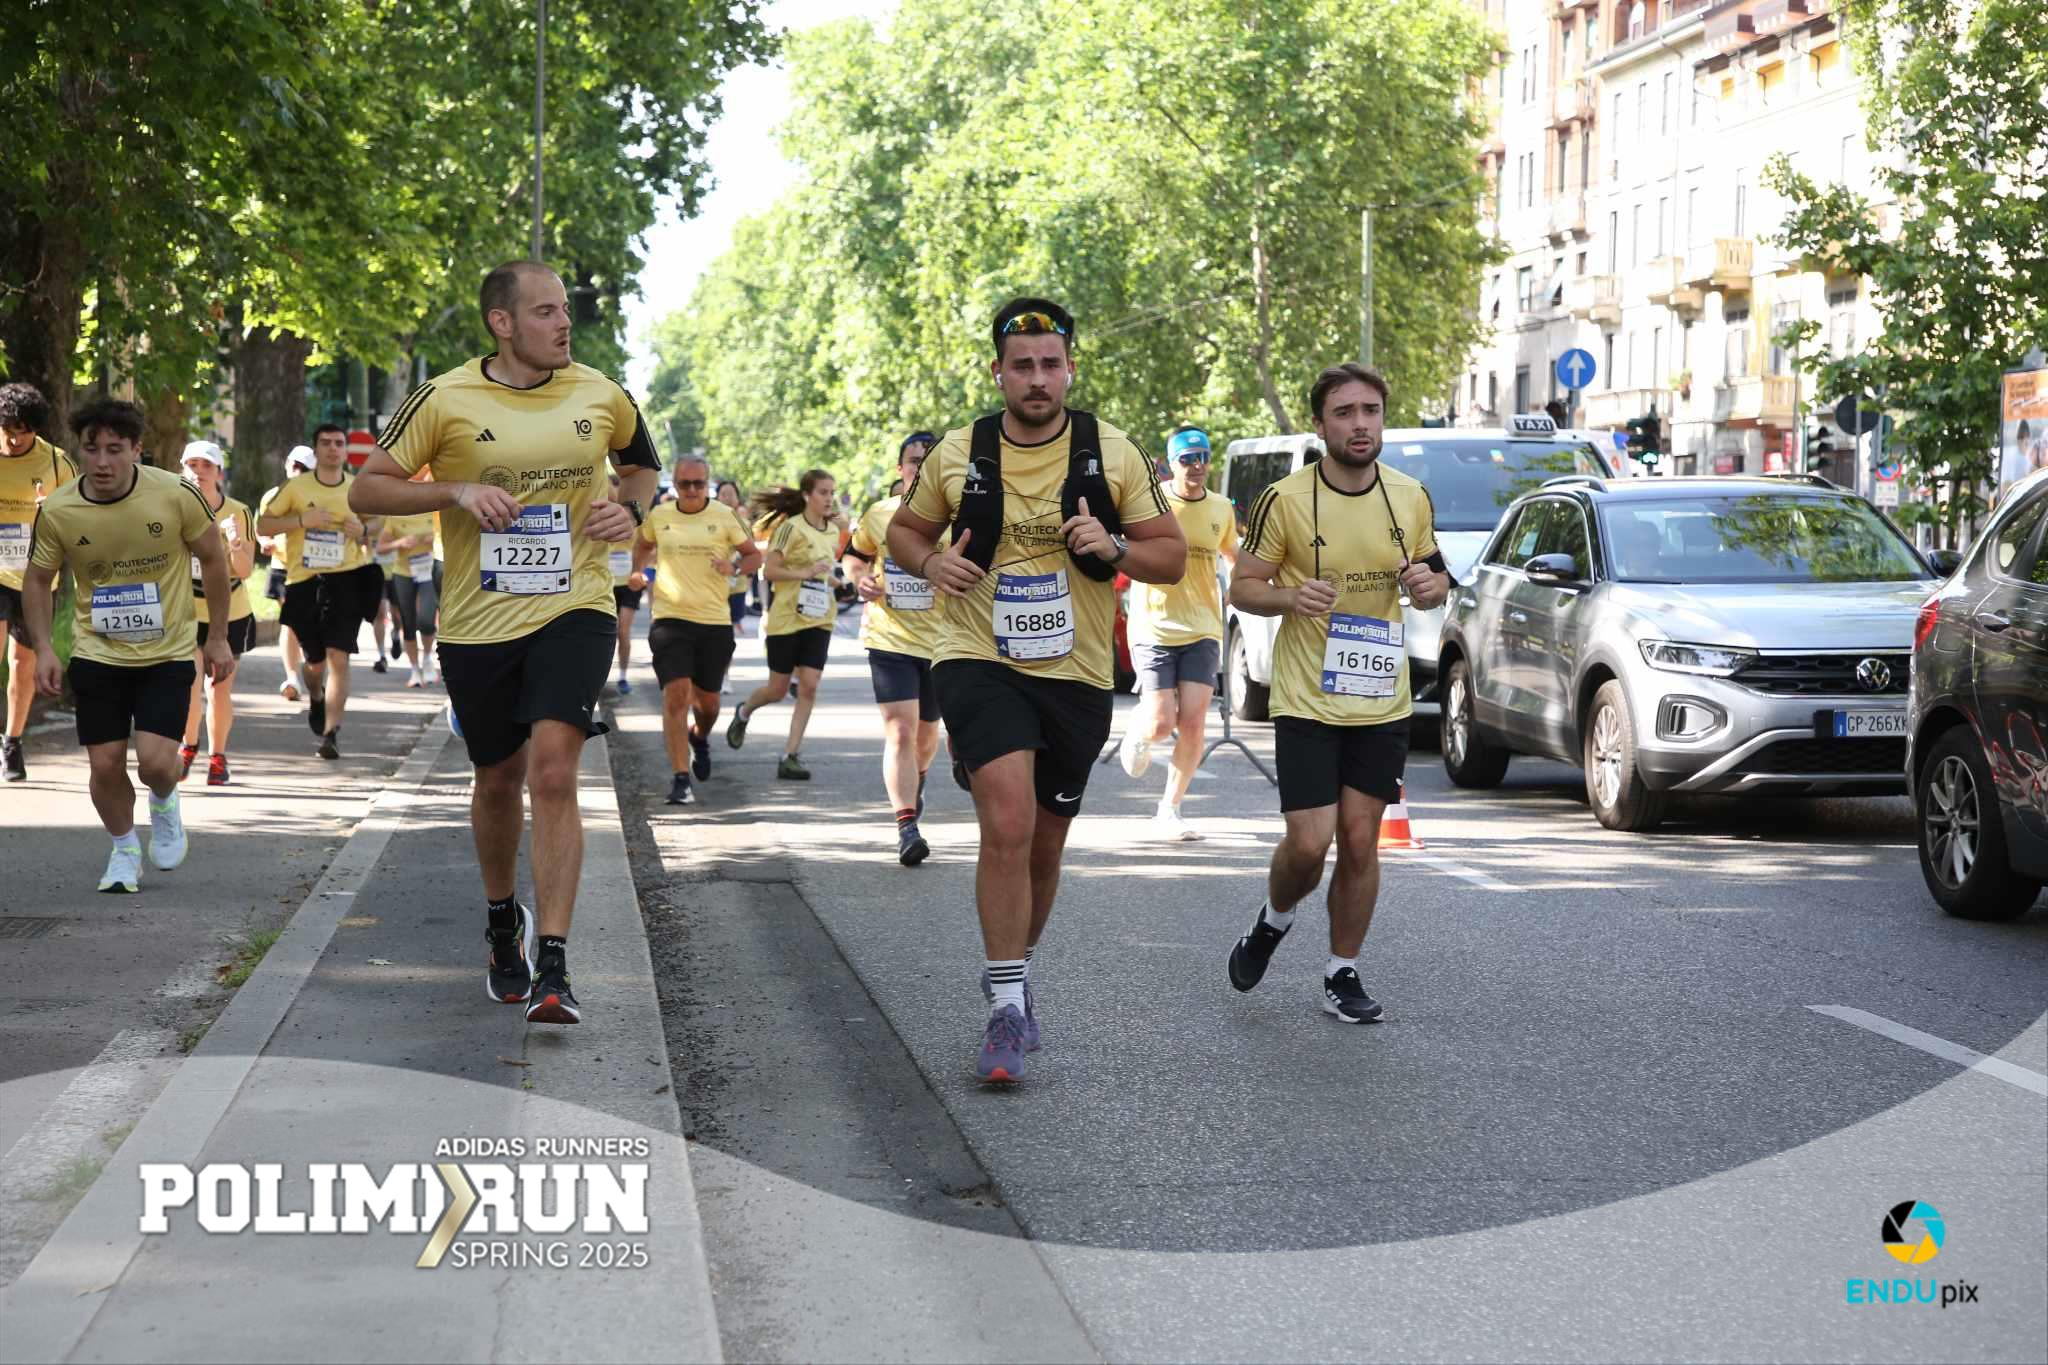
\includegraphics[width=0.5\textwidth]{fig/test/test.jpg}
    \caption{Esquema de arquitectura softwarizada.}
    \label{fig:arquitectura}
\end{figure}

\section{Tabla de prueba}

La Tabla~\ref{tab:comparativa} presenta una coparativa entre arquitecturas de red tradicionales y softwarizadas.

\begin{table}[ht]
    \centering
    \begin{tabular}{|l|c|c|}
        \hline
        \textbf{Característica} & \textbf{Tradicional} & \textbf{Softwarizada} \\
        \hline
        Flexibilidad & Baja & Alta \\
        Control Centralizado & No & Sí \\
        Automatización & Limitada & Completa \\
        \hline
    \end{tabular}
    \caption{Comparativa de arquitecturas de red.}
    \label{tab:comparativa}
\end{table}

\section{Algoritmo de prueba}

A continuación, el Algoritmo~\ref{alg:simple} muestra un pseudocódigo de ejemplo utilizando \texttt{algorithm2e}.

\begin{algorithm}[H]
\caption{Selección del nodo con mayor capacidad}
\label{alg:simple}
\SetAlgoLined
\KwIn{Lista de nodos $N$}
\KwOut{Nodo con mayor capacidad}
$maxNode \gets \text{null}$\;
$maxCap \gets 0$\;
\ForEach{$n \in N$}{
  \If{$n.capacidad > maxCap$}{
    $maxCap \gets n.capacidad$\;
    $maxNode \gets n$\;
  }
}
\Return $maxNode$\;
\end{algorithm}


%\input{body/capitulos/02_marcoteorico}
%\input{body/capitulos/03_analisisPreimplementacion}
%\input{body/capitulos/04_desarrollo}
%\input{body/capitulos/05_conclusiones}

% Biblio
%\nocite{*}
\bibliography{body/refs}
\bibliographystyle{IEEEtran}


% Anexos 
%\appendix
%\input{body/anexos/condiciones}
%\input{body/anexos/presupuesto}
%\input{body/anexos/manuales}


% Contra portada
%\includepdf[pages={4}]{include/portada/portada_uah_eps_MUIT_TFM.pdf}
%\includepdf[pages={6}]{include/portada/portada_uah_eps_MUIT_TFM.pdf}

\end{document}